\documentclass{beamer}
\usetheme{Madrid}
\usecolortheme{default}
\usepackage{graphicx}
\usepackage{booktabs}
\usepackage{multirow}
\usepackage{amsmath}
\usepackage{hyperref}
\usepackage{xcolor}

% Define colors
\definecolor{outlineblue}{RGB}{44, 48, 148}
\definecolor{outlinegray}{RGB}{200, 200, 215}

% Custom command for outline slides
\newcommand{\customoutline}[1]{%
\begin{frame}
\frametitle{\textcolor{white}{Outline}}
\setbeamercolor{frametitle}{bg=outlineblue, fg=white}
\vspace{0.5cm}
\begin{itemize}
\setlength{\itemsep}{0.8em}
\item[\ifnum1=#1\textcolor{outlineblue}{$\bullet$}\else\textcolor{outlinegray}{$\circ$}\fi] \ifnum1=#1\textcolor{outlineblue}{1 Introduction}\else\textcolor{outlinegray}{1 Introduction}\fi
\item[\ifnum2=#1\textcolor{outlineblue}{$\bullet$}\else\textcolor{outlinegray}{$\circ$}\fi] \ifnum2=#1\textcolor{outlineblue}{2 Background}\else\textcolor{outlinegray}{2 Background}\fi
\item[\ifnum3=#1\textcolor{outlineblue}{$\bullet$}\else\textcolor{outlinegray}{$\circ$}\fi] \ifnum3=#1\textcolor{outlineblue}{3 Methodology}\else\textcolor{outlinegray}{3 Methodology}\fi
\item[\ifnum4=#1\textcolor{outlineblue}{$\bullet$}\else\textcolor{outlinegray}{$\circ$}\fi] \ifnum4=#1\textcolor{outlineblue}{4 Results}\else\textcolor{outlinegray}{4 Results}\fi
\item[\ifnum5=#1\textcolor{outlineblue}{$\bullet$}\else\textcolor{outlinegray}{$\circ$}\fi] \ifnum5=#1\textcolor{outlineblue}{5 Conclusions}\else\textcolor{outlinegray}{5 Conclusions}\fi
\end{itemize}
\end{frame}
}

% Change frame title colors
\setbeamercolor{frametitle}{bg=outlineblue, fg=white}
\setbeamercolor{title}{bg=outlineblue, fg=white}

\title{Two-Stage Emotion Detection from Multimodal Data}
\author{Xiangyi Li}
\institute{San José State University\\Department of Computer Science}
\date{Spring 2024}

\begin{document}

% Title page
\begin{frame}
\titlepage
\end{frame}

% Initial outline showing all sections
\customoutline{0}

% Introduction section
\customoutline{1}
\section{Introduction}

\begin{frame}
\frametitle{Introduction}
\begin{itemize}
    \item \textbf{Emotion detection} is crucial for human-computer interaction
    \item Enables machines to recognize and respond to human emotional states
    \item Applications:
    \begin{itemize}
        \item Mental health monitoring
        \item Customer service
        \item Human-computer interaction
        \item Sentiment analysis
    \end{itemize}
    \item \textbf{Challenge}: Emotions are complex, multidimensional phenomena
    \item \textbf{Scale of Research}: \alert{392 experiments} conducted using \alert{10 H100 GPUs} from Modal.com
\end{itemize}
\end{frame}

\begin{frame}
\frametitle{Problem Statement}
\begin{itemize}
    \item \textbf{Current Limitations}:
    \begin{itemize}
        \item Emotion detection often treats emotions as discrete categories only
        \item Limited understanding of the relationship between dimensional and categorical emotion models
        \item Insufficient exploration of the relative contributions of text vs. audio modalities
        \item Lack of comprehensive comparison of fusion strategies
    \end{itemize}
    \item \textbf{Proposed Solution}:
    \begin{itemize}
        \item Two-stage approach: dimensional prediction → categorical mapping
        \item Comprehensive evaluation of multimodal fusion techniques
        \item Extensive experimentation with state-of-the-art models
    \end{itemize}
\end{itemize}
\end{frame}

\begin{frame}
\frametitle{Research Questions}
\begin{enumerate}
    \item How does a \textbf{two-stage approach} (dimensional prediction → category mapping) compare to \textbf{direct classification} for emotion recognition?
    \item What is the relative contribution of \textbf{text vs. audio modalities} for emotion detection?
    \item Which \textbf{fusion strategies} best integrate multimodal information?
    \item How do different \textbf{transformer architectures} perform for emotion detection tasks?
\end{enumerate}
\end{frame}

\begin{frame}
\frametitle{Significance and Contributions}
\begin{itemize}
    \item \textbf{Theoretical Contributions}:
    \begin{itemize}
        \item New insights into the relationship between dimensional and categorical emotion models
        \item Understanding of modality-specific contributions to different emotion dimensions
    \end{itemize}
    \item \textbf{Technical Contributions}:
    \begin{itemize}
        \item Novel two-stage approach for emotion detection
        \item Comprehensive evaluation of fusion strategies
        \item Performance benchmarks for state-of-the-art models
    \end{itemize}
    \item \textbf{Practical Contributions}:
    \begin{itemize}
        \item Guidelines for selecting appropriate models and approaches for specific applications
        \item Insights into performance-efficiency tradeoffs
    \end{itemize}
\end{itemize}
\end{frame}

\begin{frame}
\frametitle{Research Scope and Limitations}
\begin{itemize}
    \item \textbf{Focus}:
    \begin{itemize}
        \item Text and audio modalities (excluding visual)
        \item English language content
        \item Six basic emotions plus neutral state
    \end{itemize}
    \item \textbf{Dataset}:
    \begin{itemize}
        \item IEMOCAP (Interactive Emotional Dyadic Motion Capture)
        \item 12 hours of audio-visual conversations between 10 speakers
        \item Both categorical and dimensional annotations
    \end{itemize}
    \item \textbf{Limitations}:
    \begin{itemize}
        \item Cultural diversity not fully represented
        \item Limited to acted emotions rather than spontaneous expressions
        \item Does not address privacy concerns in real-world applications
    \end{itemize}
\end{itemize}
\end{frame}

% Background section
\customoutline{2}
\section{Background}

\begin{frame}
\frametitle{Dimensional vs. Categorical Emotion Models}
\begin{columns}
\column{0.5\textwidth}
\textbf{Dimensional Model}
\begin{itemize}
    \item Represents emotions as points in continuous space
    \item \textbf{AVD dimensions}:
    \begin{itemize}
        \item \textbf{A}rousal: energy/intensity
        \item \textbf{V}alence: positive/negative
        \item \textbf{D}ominance: control/power
    \end{itemize}
    \item Captures nuanced emotional states
\end{itemize}

\column{0.5\textwidth}
\textbf{Categorical Model}
\begin{itemize}
    \item Discrete emotion labels (anger, joy, sadness, etc.)
    \item Easier to classify
    \item More intuitive for humans
    \item Less granular representation
\end{itemize}
\end{columns}

\begin{center}
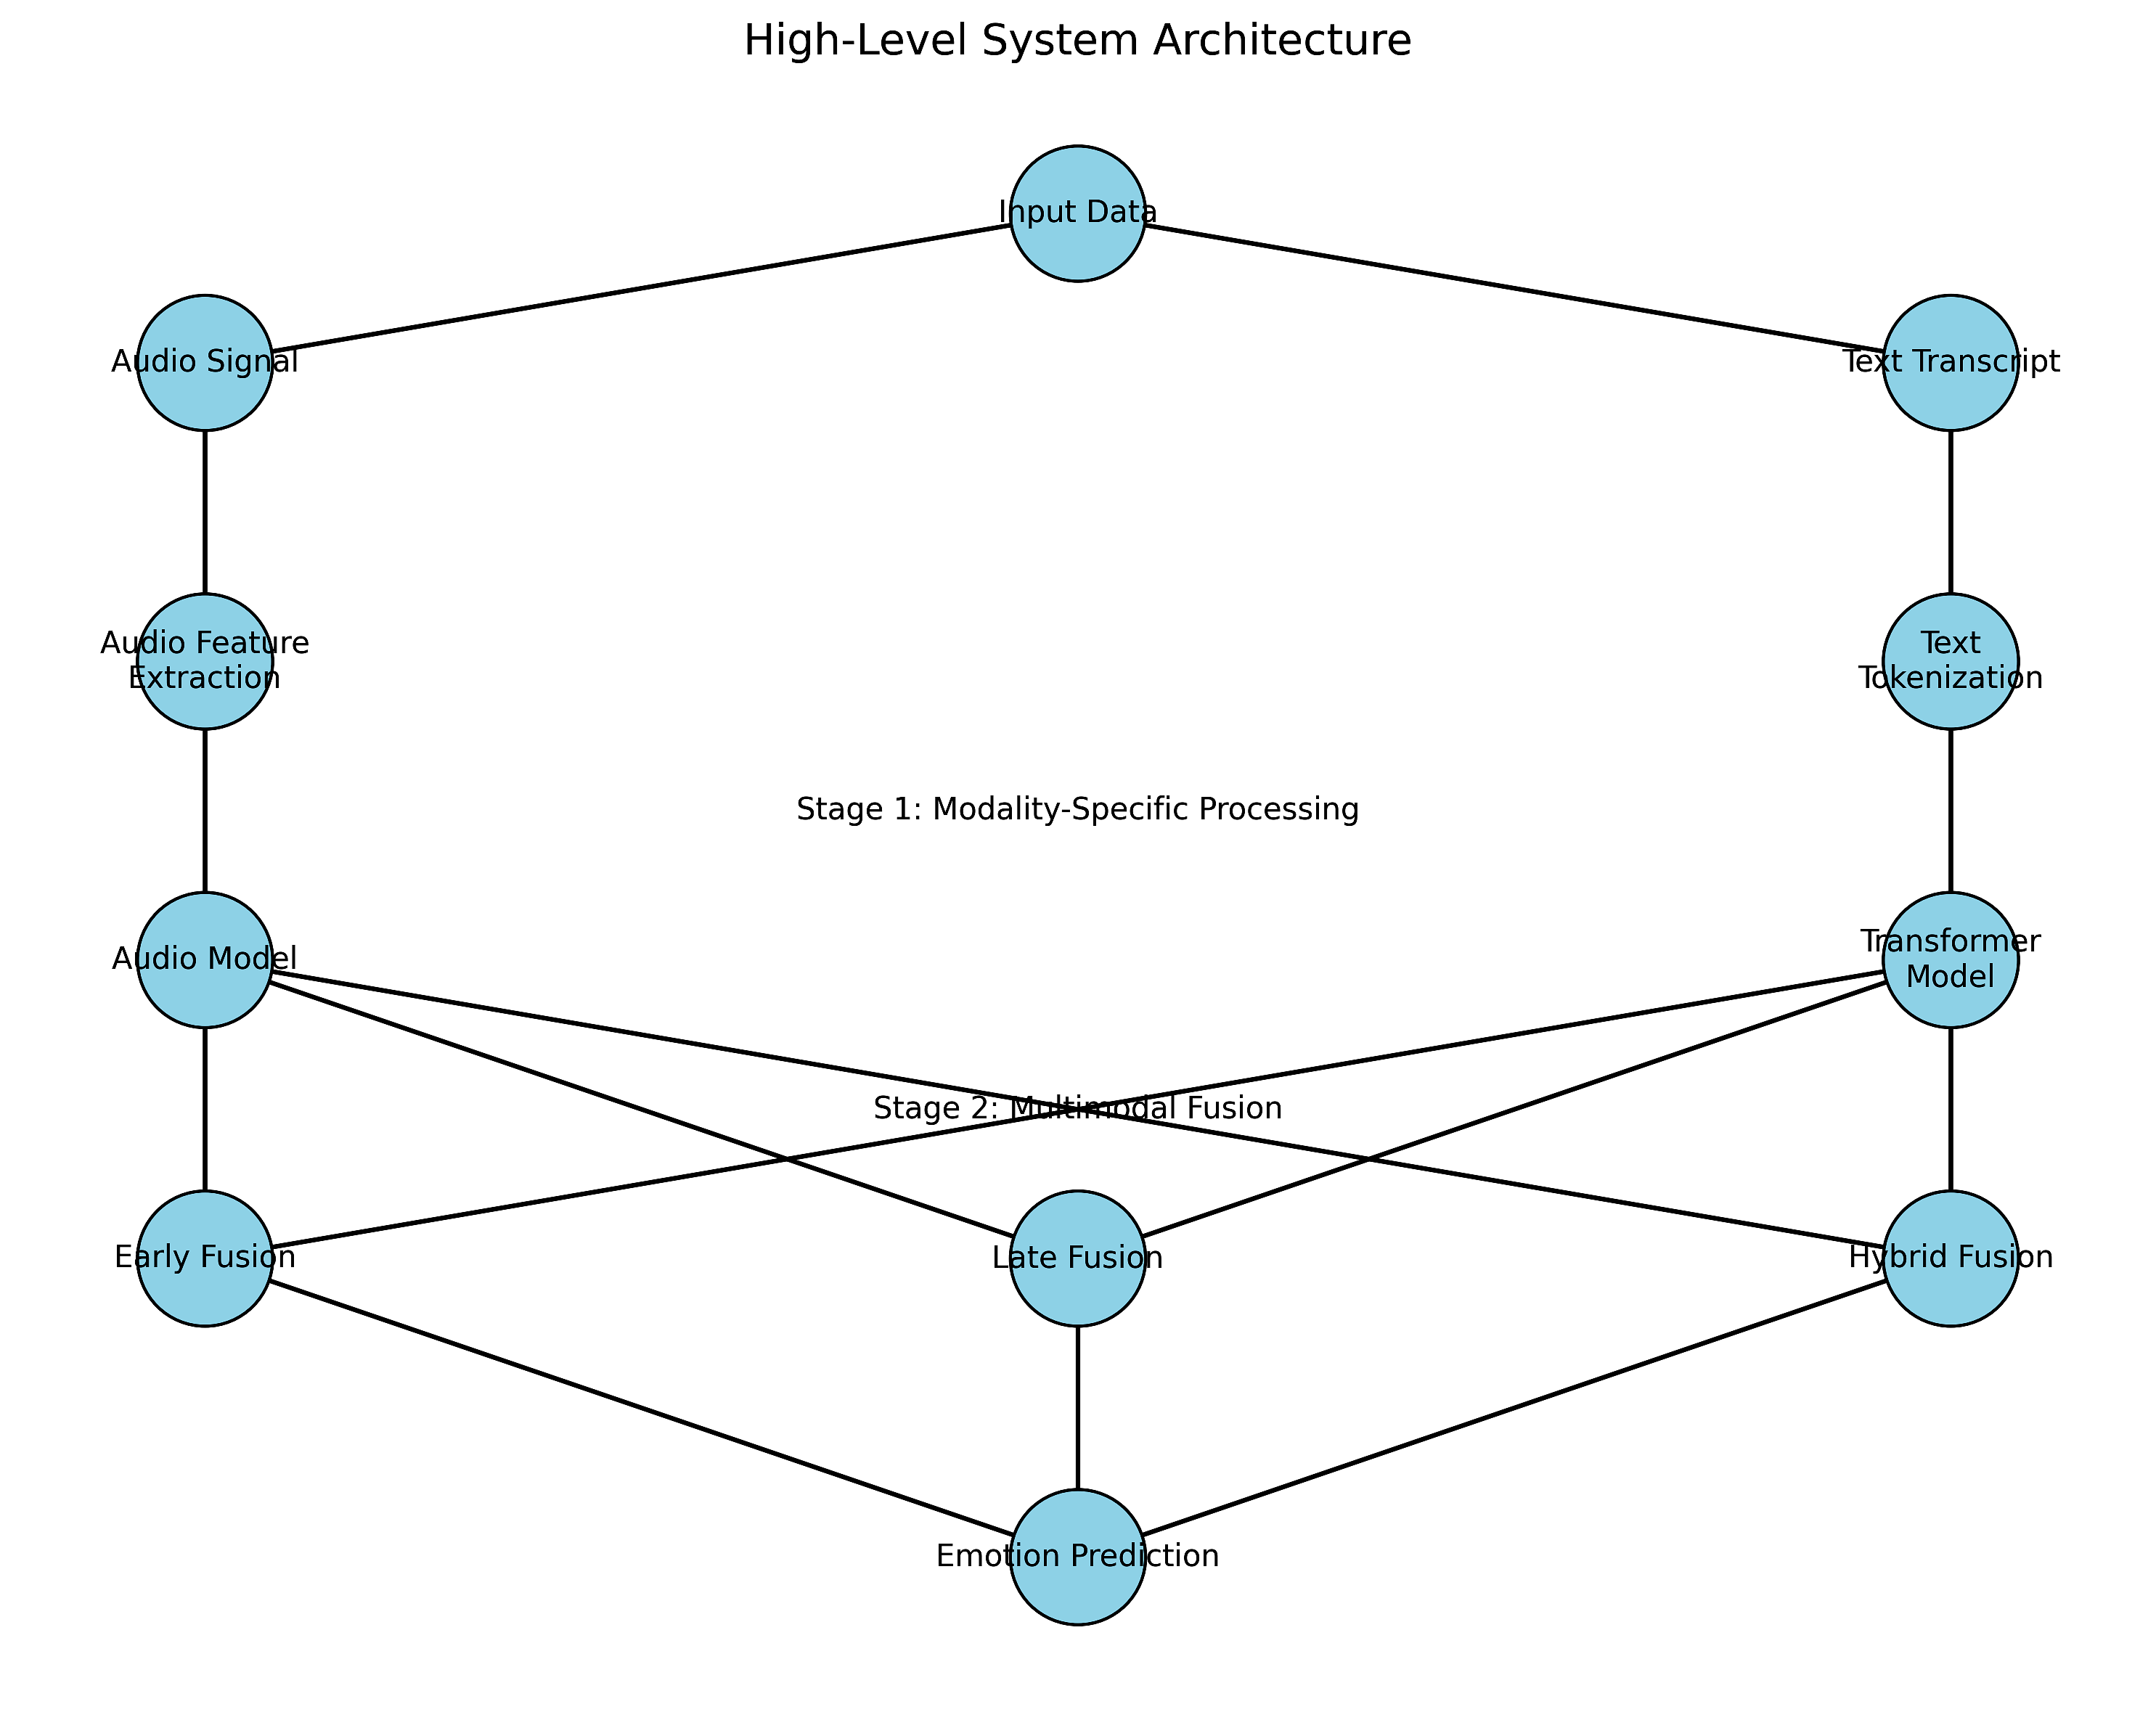
\includegraphics[width=0.5\textwidth]{figures/system_architecture.png}
\end{center}
\end{frame}

\begin{frame}
\frametitle{Dimensional Emotion Space}
\begin{columns}
\column{0.6\textwidth}
\begin{itemize}
    \item \textbf{Valence-Arousal Space}:
    \begin{itemize}
        \item Valence: horizontal axis (negative to positive)
        \item Arousal: vertical axis (low to high energy)
    \end{itemize}
    \item \textbf{Examples}:
    \begin{itemize}
        \item Anger: negative valence, high arousal
        \item Joy: positive valence, high arousal
        \item Sadness: negative valence, low arousal
        \item Contentment: positive valence, low arousal
    \end{itemize}
\end{itemize}

\column{0.4\textwidth}
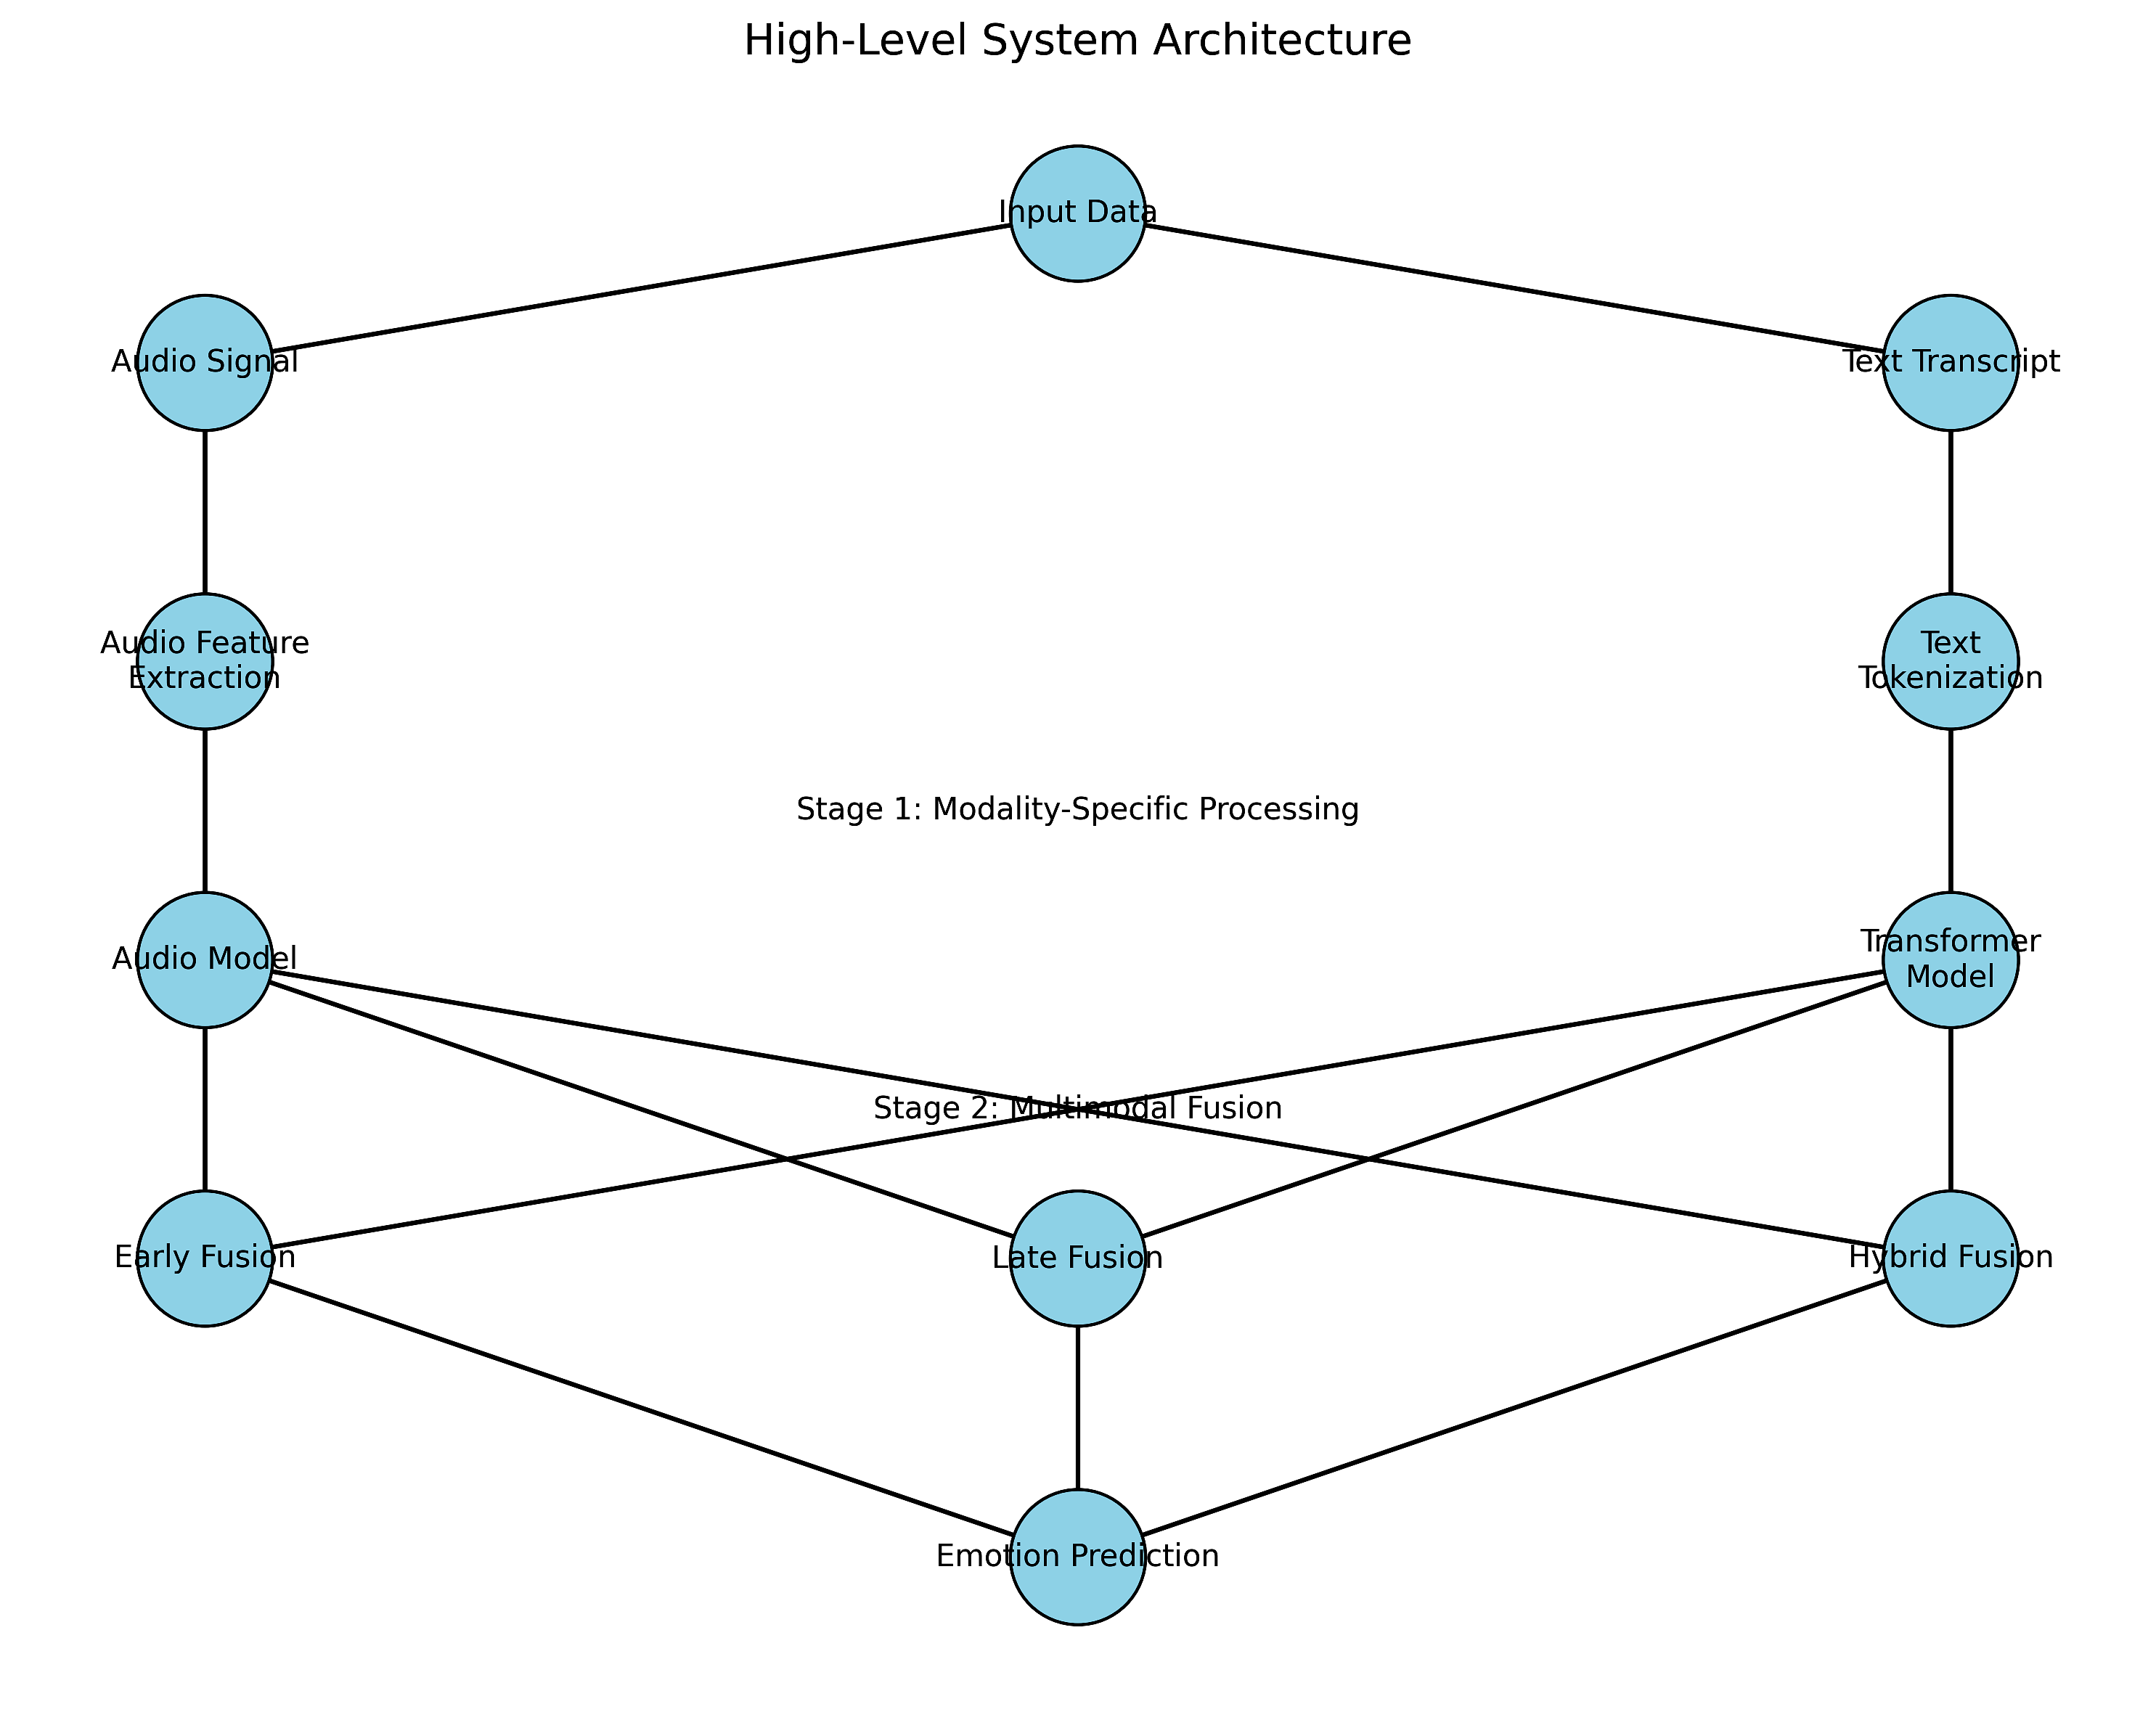
\includegraphics[width=\textwidth]{figures/system_architecture.png}
\end{columns}
\end{frame}

\begin{frame}
\frametitle{Mapping Between Models}
\begin{itemize}
    \item \textbf{Mapping Dimensional → Categorical}:
    \begin{itemize}
        \item Regions in AVD space can be mapped to discrete categories
        \item Fuzzy boundaries between categories
        \item Some points may represent blended emotions
    \end{itemize}
    \item \textbf{Advantages of Two-Stage Approach}:
    \begin{itemize}
        \item Captures emotional intensity
        \item Recognizes nuanced/mixed emotional states
        \item Provides more information for downstream tasks
        \item Potentially more generalizable across cultures
    \end{itemize}
    \item \textbf{Challenges}:
    \begin{itemize}
        \item Increased complexity
        \item Error propagation between stages
        \item Need for dimensional annotations
    \end{itemize}
\end{itemize}
\end{frame}

\begin{frame}
\frametitle{Evolution of Emotion Recognition}
\begin{itemize}
    \item \textbf{Pre-2012}: Mostly rule-based systems and traditional ML
    \begin{itemize}
        \item SVM, Decision Trees, Bayesian methods
        \item Handcrafted features like lexicons and acoustic parameters
    \end{itemize}
    \item \textbf{Deep Learning Era (2013-2017)}: 
    \begin{itemize}
        \item CNNs, RNNs for feature extraction
        \item Word embeddings (Word2Vec, GloVe)
    \end{itemize}
    \item \textbf{Transformer Era (2018-Present)}:
    \begin{itemize}
        \item BERT, RoBERTa, XLNet, DeBERTa
        \item Attention-based architectures enable better context modeling
    \end{itemize}
\end{itemize}
\end{frame}

\begin{frame}
\frametitle{Transformer Architecture Overview}
\begin{columns}
\column{0.5\textwidth}
\begin{itemize}
    \item \textbf{Key Innovations}:
    \begin{itemize}
        \item Self-attention mechanism
        \item Parallelizable architecture
        \item Contextual representations
        \item Pre-training and fine-tuning paradigm
    \end{itemize}
    \item \textbf{Advantages for Emotion Detection}:
    \begin{itemize}
        \item Captures long-range dependencies
        \item Models context effectively
        \item Captures subtle emotional cues
    \end{itemize}
\end{itemize}

\column{0.5\textwidth}
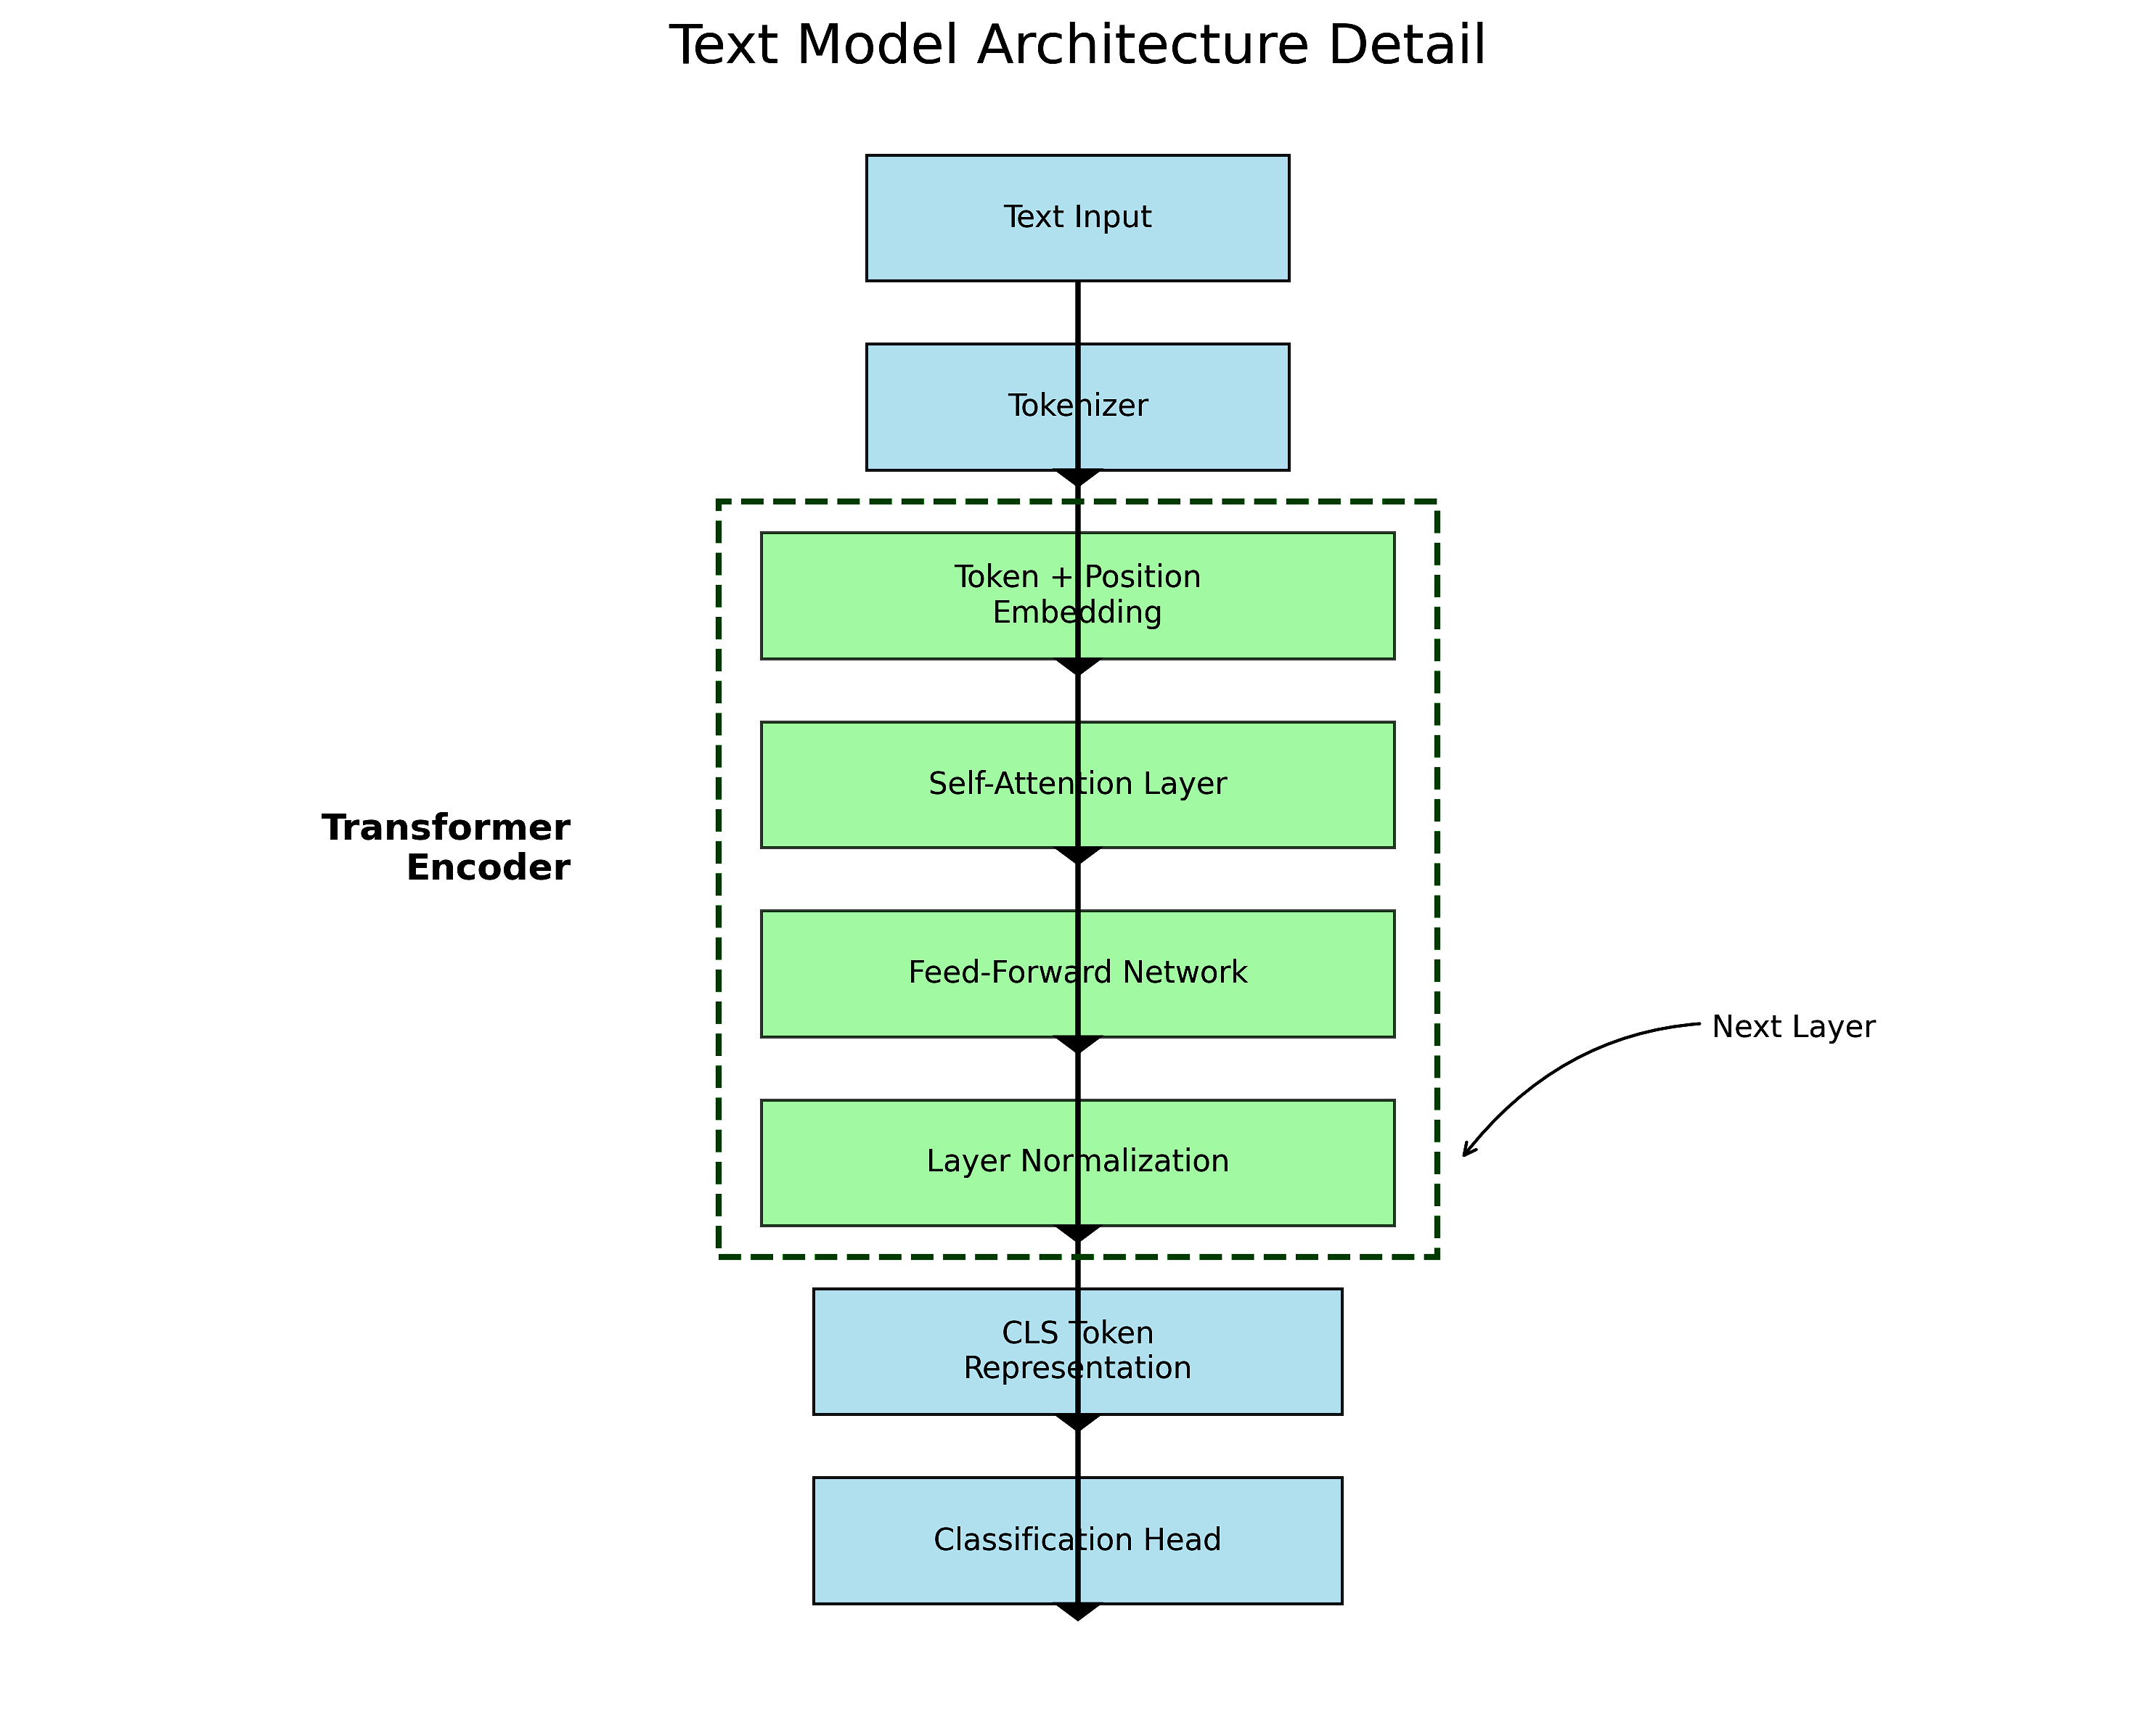
\includegraphics[width=\textwidth]{figures/text_model_architecture.png}
\end{columns}
\end{frame}

\begin{frame}
\frametitle{Multimodal Emotion Recognition}
\begin{itemize}
    \item \textbf{Complementary Information}:
    \begin{itemize}
        \item Text: semantic content, explicit statements
        \item Audio: prosodic features, intensity, emotional tone
        \item Visual: facial expressions, gestures, body language
    \end{itemize}
    \item \textbf{Challenges in Multimodal Integration}:
    \begin{itemize}
        \item Alignment of modalities
        \item Different sampling rates and feature dimensions
        \item Handling missing modalities
        \item Optimal fusion strategies
    \end{itemize}
    \item \textbf{Potential Benefits}:
    \begin{itemize}
        \item More robust detection
        \item Capture of complementary emotional signals
        \item Higher accuracy across diverse contexts
    \end{itemize}
\end{itemize}
\end{frame}

\begin{frame}
\frametitle{Current Challenges in Emotion Detection}
\begin{columns}
\column{0.5\textwidth}
\begin{itemize}
    \item \textbf{Technical Challenges}:
    \begin{itemize}
        \item Fusion of heterogeneous data
        \item Real-time processing requirements
        \item Model size vs. performance tradeoffs
    \end{itemize}
    \item \textbf{Data Challenges}:
    \begin{itemize}
        \item Limited annotated datasets
        \item Subjectivity in emotion labeling
        \item Cultural and individual differences
    \end{itemize}
\end{itemize}

\column{0.5\textwidth}
\begin{itemize}
    \item \textbf{Research Gaps}:
    \begin{itemize}
        \item Limited work on dimensional-categorical mapping
        \item Few comprehensive comparisons of fusion strategies
        \item Insufficient exploration of modality contributions
    \end{itemize}
    \item \textbf{Ethical Concerns}:
    \begin{itemize}
        \item Privacy implications
        \item Potential for misuse
        \item Bias in emotion recognition
    \end{itemize}
\end{itemize}
\end{columns}
\end{frame}

% Methodology section
\customoutline{3}
\section{Methodology}

\begin{frame}
\frametitle{System Architecture}
\begin{center}
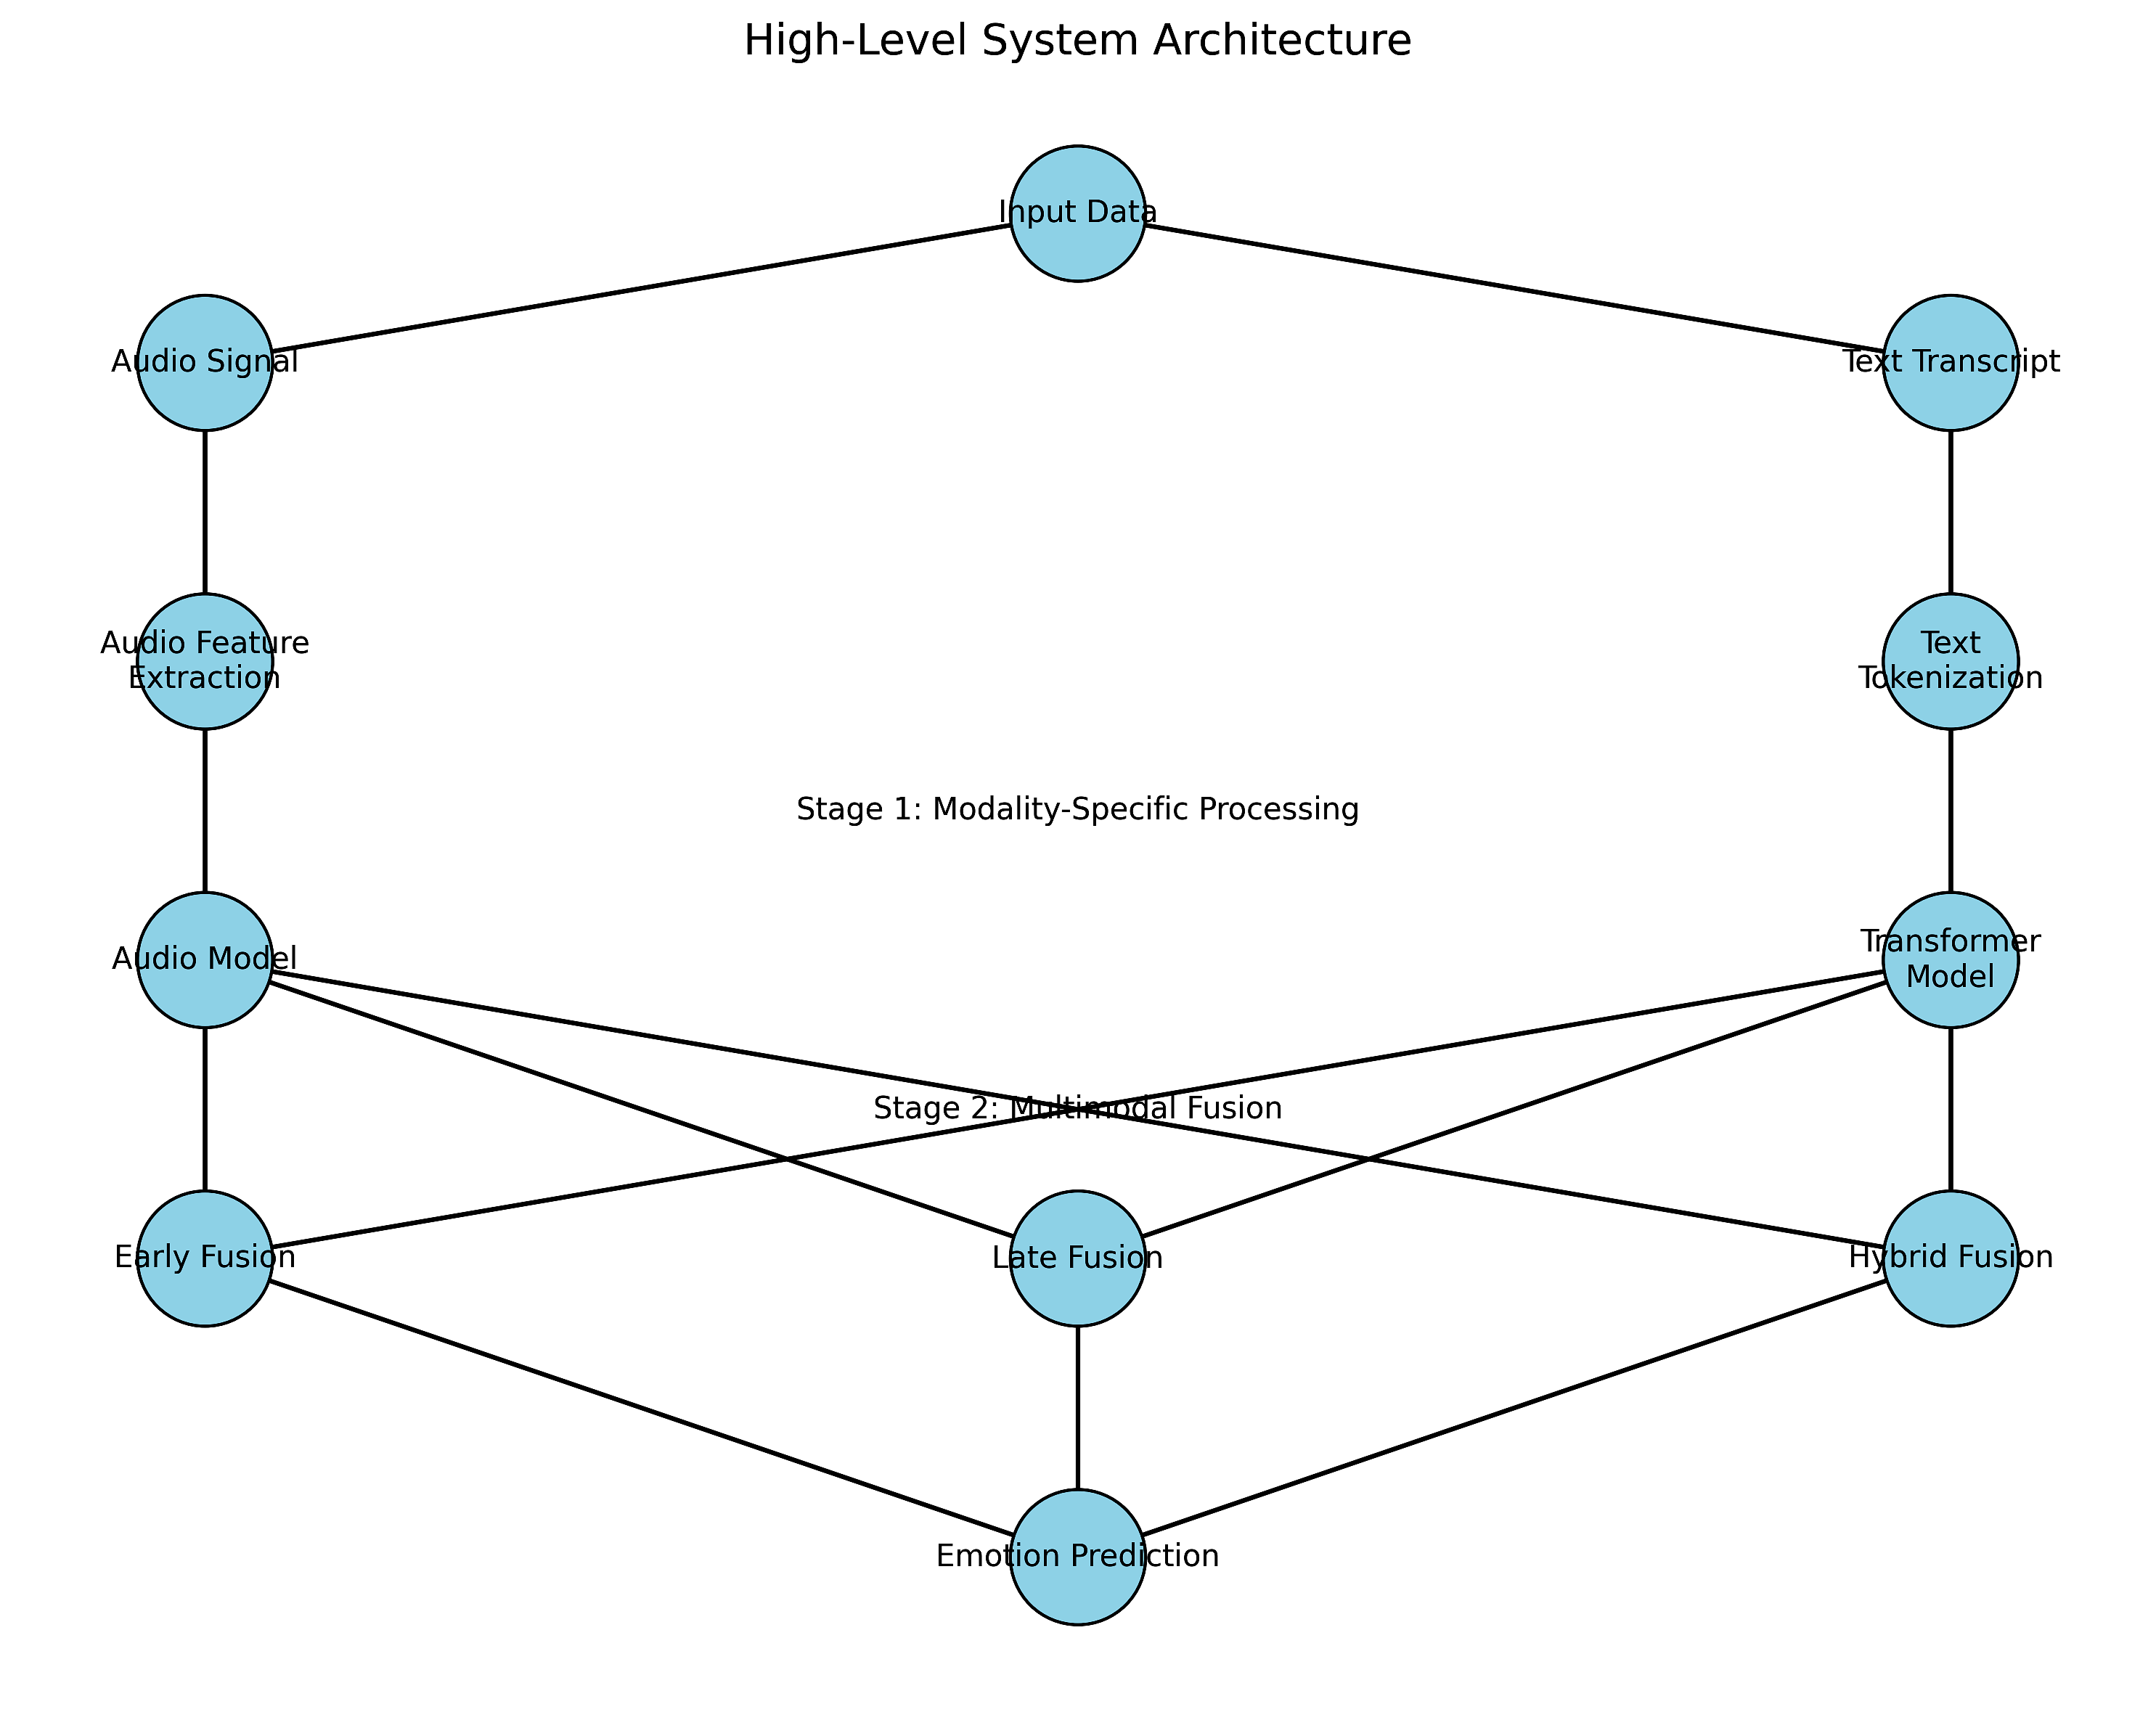
\includegraphics[width=0.9\textwidth]{figures/system_architecture.png}
\end{center}

\begin{itemize}
    \item \textbf{Stage 1}: Predict dimensional values (Arousal, Valence, Dominance)
    \item \textbf{Stage 2}: Map dimensional values to categorical emotions
\end{itemize}
\end{frame}

\begin{frame}
\frametitle{Text Processing Models}
\begin{center}
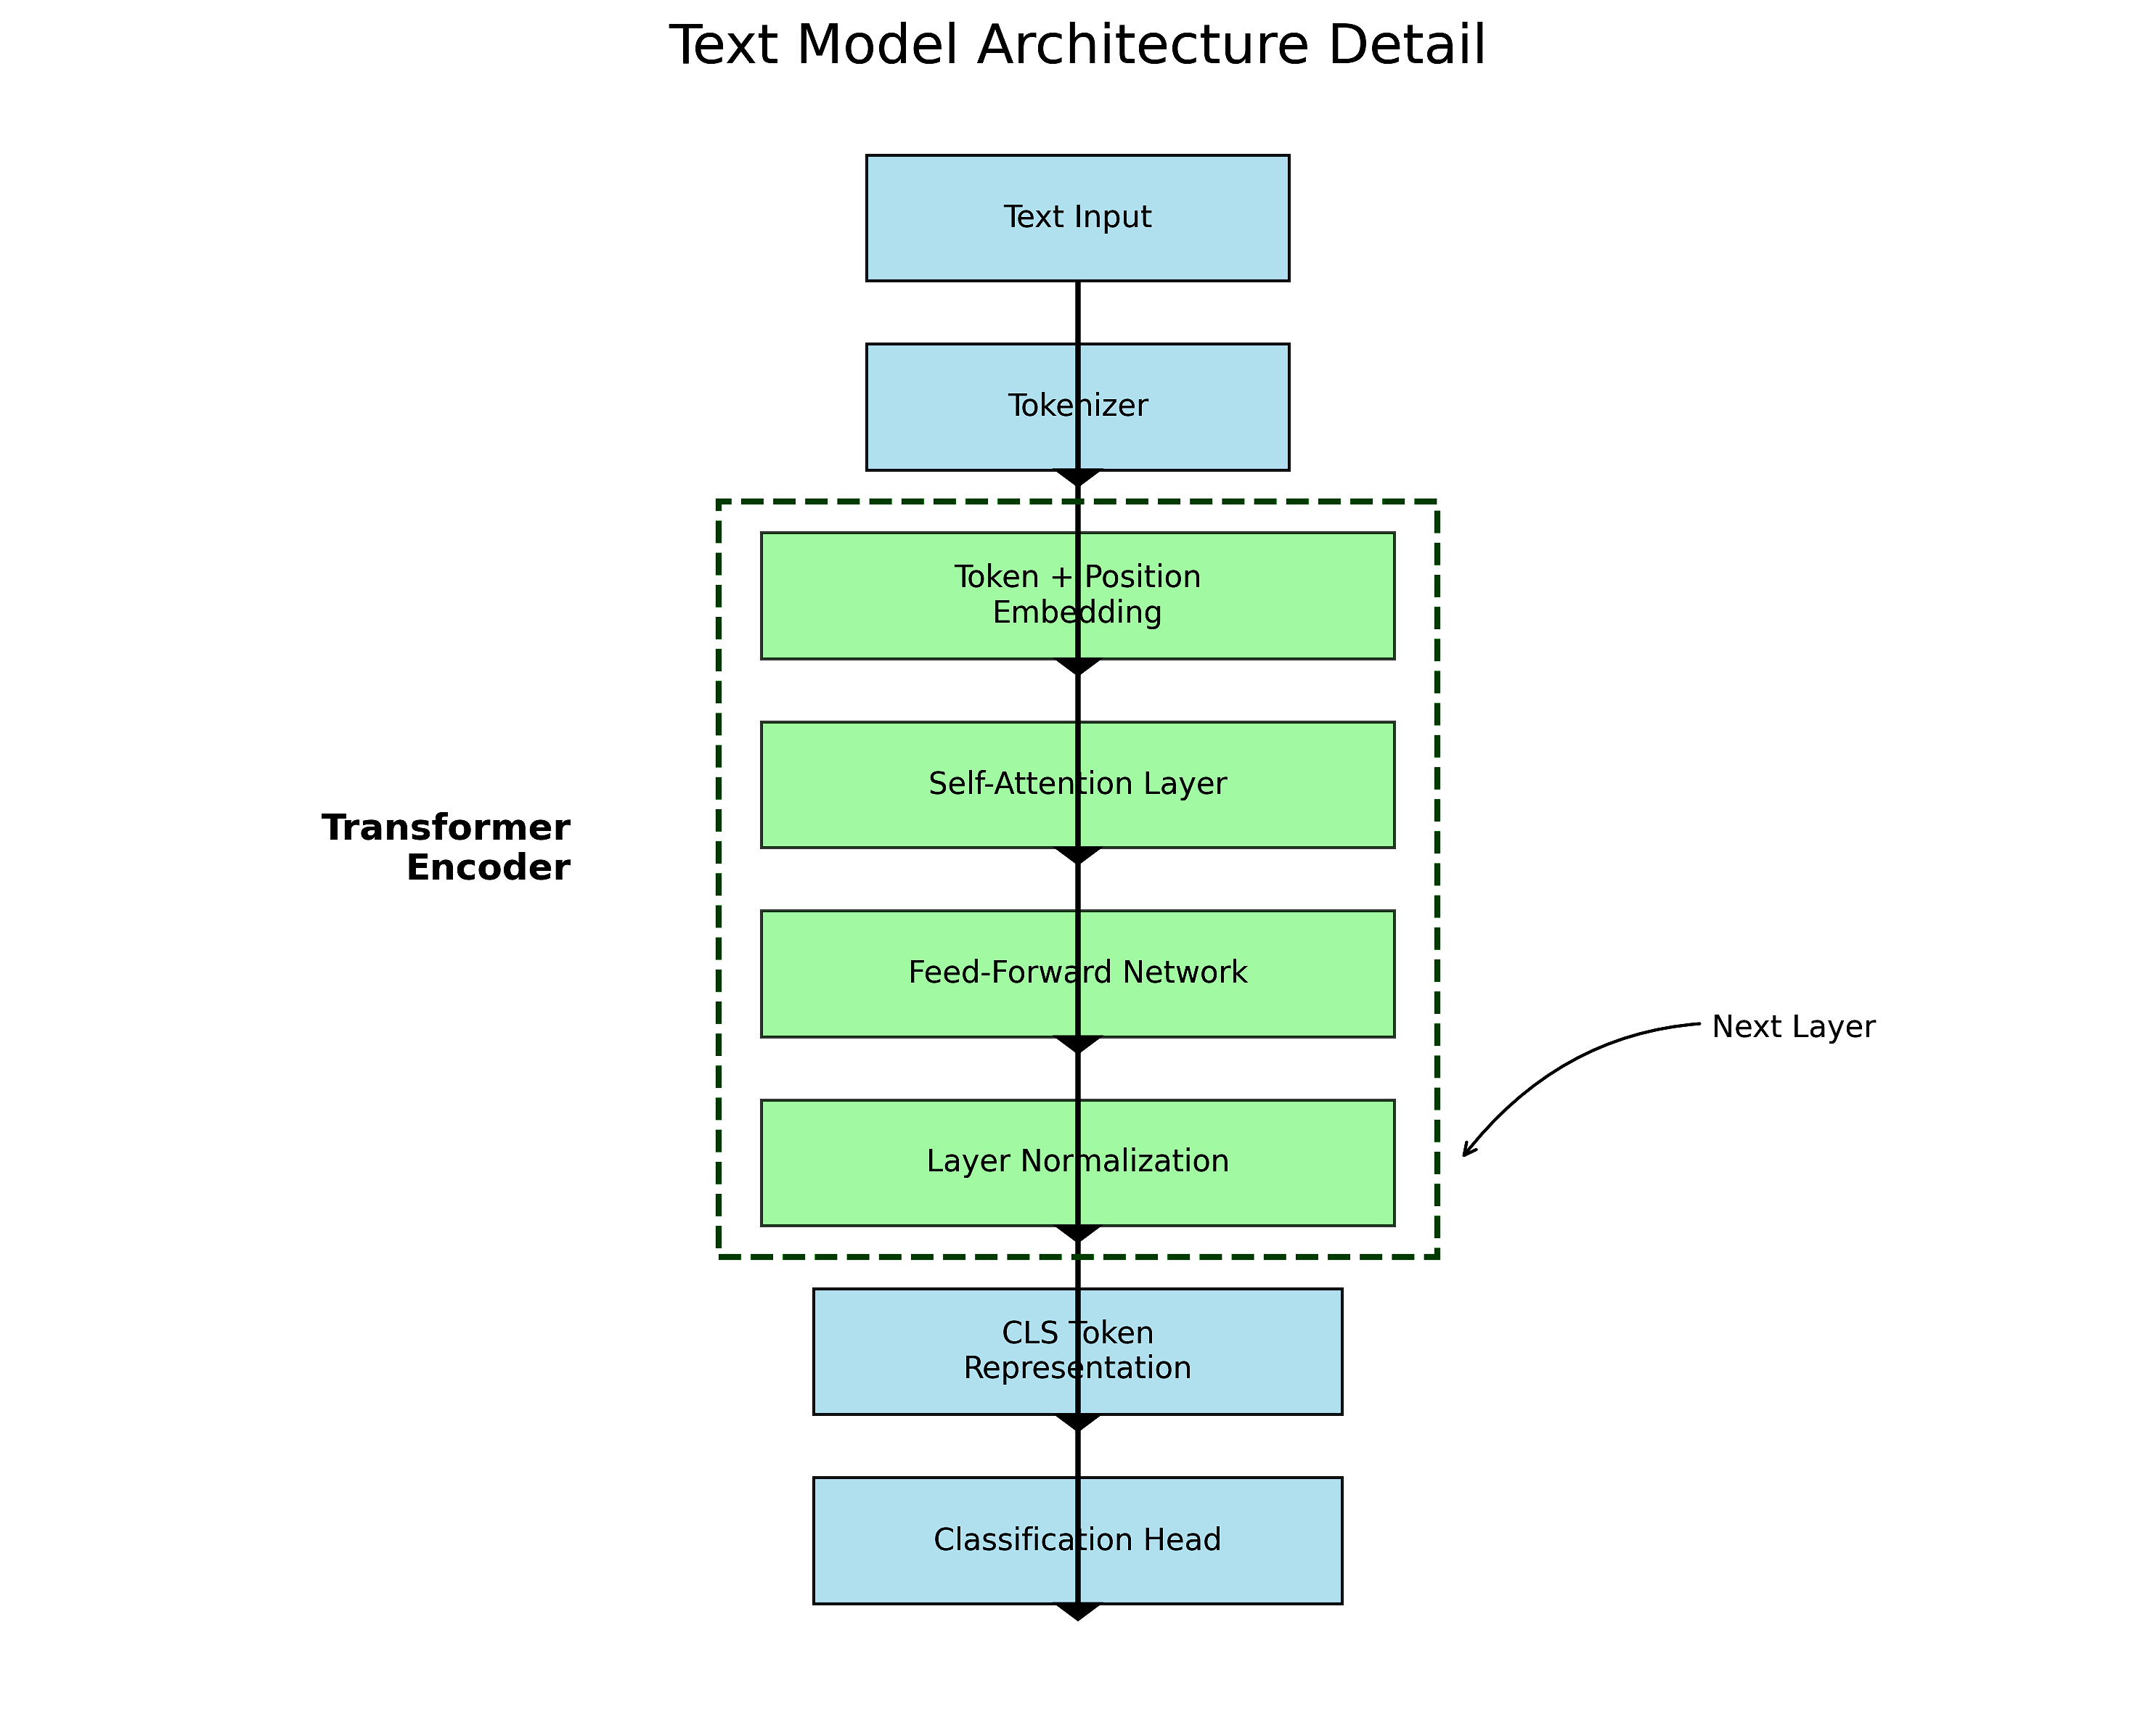
\includegraphics[width=0.9\textwidth]{figures/text_model_architecture.png}
\end{center}

\begin{itemize}
    \item \textbf{BERT}: Bidirectional context modeling (110M parameters)
    \item \textbf{RoBERTa}: Optimized BERT with larger corpus (125M parameters)
    \item \textbf{XLNet}: Autoregressive pretraining
    \item \textbf{ALBERT}: Parameter-efficient BERT variant
    \item \textbf{ELECTRA}: Generator-discriminator pretraining
    \item \textbf{DeBERTa}: Disentangled attention mechanism
\end{itemize}
\end{frame}

\begin{frame}
\frametitle{BERT Architecture Details}
\begin{columns}
\column{0.5\textwidth}
\begin{itemize}
    \item \textbf{Structure}:
    \begin{itemize}
        \item 12 transformer encoder layers
        \item 768 hidden dimensions
        \item 12 attention heads
        \item 110M parameters
    \end{itemize}
    \item \textbf{Pre-training Objectives}:
    \begin{itemize}
        \item Masked Language Modeling (MLM)
        \item Next Sentence Prediction (NSP)
    \end{itemize}
\end{itemize}

\column{0.5\textwidth}
\begin{itemize}
    \item \textbf{Fine-tuning for Emotion Detection}:
    \begin{itemize}
        \item Use [CLS] token representation
        \item Add regression head for AVD prediction
        \item Add classification head for direct classification
    \end{itemize}
    \item \textbf{Input Processing}:
    \begin{itemize}
        \item Tokenization
        \item Special token addition ([CLS], [SEP])
        \item Max sequence length: 512 tokens
    \end{itemize}
\end{itemize}
\end{columns}
\end{frame}

\begin{frame}
\frametitle{RoBERTa Improvements over BERT}
\begin{itemize}
    \item \textbf{Training Methodology Improvements}:
    \begin{itemize}
        \item Removed Next Sentence Prediction objective
        \item Dynamic masking instead of static masking
        \item Trained with larger batches (8K sequences)
        \item 10x more training data (160GB vs. 16GB)
        \item Longer sequences during training
    \end{itemize}
    \item \textbf{Implementation Details}:
    \begin{itemize}
        \item Same architecture as BERT-base (12 layers, 768 hidden)
        \item Byte-level BPE with 50,265 token vocabulary
        \item Total parameters: 125M
    \end{itemize}
    \item \textbf{Performance Gains}:
    \begin{itemize}
        \item More robust representations
        \item Better performance on downstream tasks
        \item Improved handling of nuanced emotional content
    \end{itemize}
\end{itemize}
\end{frame}

\begin{frame}
\frametitle{Advanced Transformer Variants}
\begin{columns}
\column{0.5\textwidth}
\textbf{XLNet}:
\begin{itemize}
    \item Permutation-based training
    \item Autoregressive formulation
    \item Captures bidirectional context without masking
    \item Better long-range dependencies
\end{itemize}

\textbf{ALBERT}:
\begin{itemize}
    \item Parameter reduction techniques
    \item Cross-layer parameter sharing
    \item Factorized embedding parameterization
    \item Sentence ordering objective
\end{itemize}

\column{0.5\textwidth}
\textbf{ELECTRA}:
\begin{itemize}
    \item Generator-discriminator architecture
    \item Replaced token detection objective
    \item More efficient training
    \item Better sample efficiency
\end{itemize}

\textbf{DeBERTa}:
\begin{itemize}
    \item Disentangled attention mechanism
    \item Enhanced mask decoder
    \item Separate content and position attention
    \item State-of-the-art performance
\end{itemize}
\end{columns}
\end{frame}

\begin{frame}
\frametitle{Audio Feature Extraction}
\begin{center}
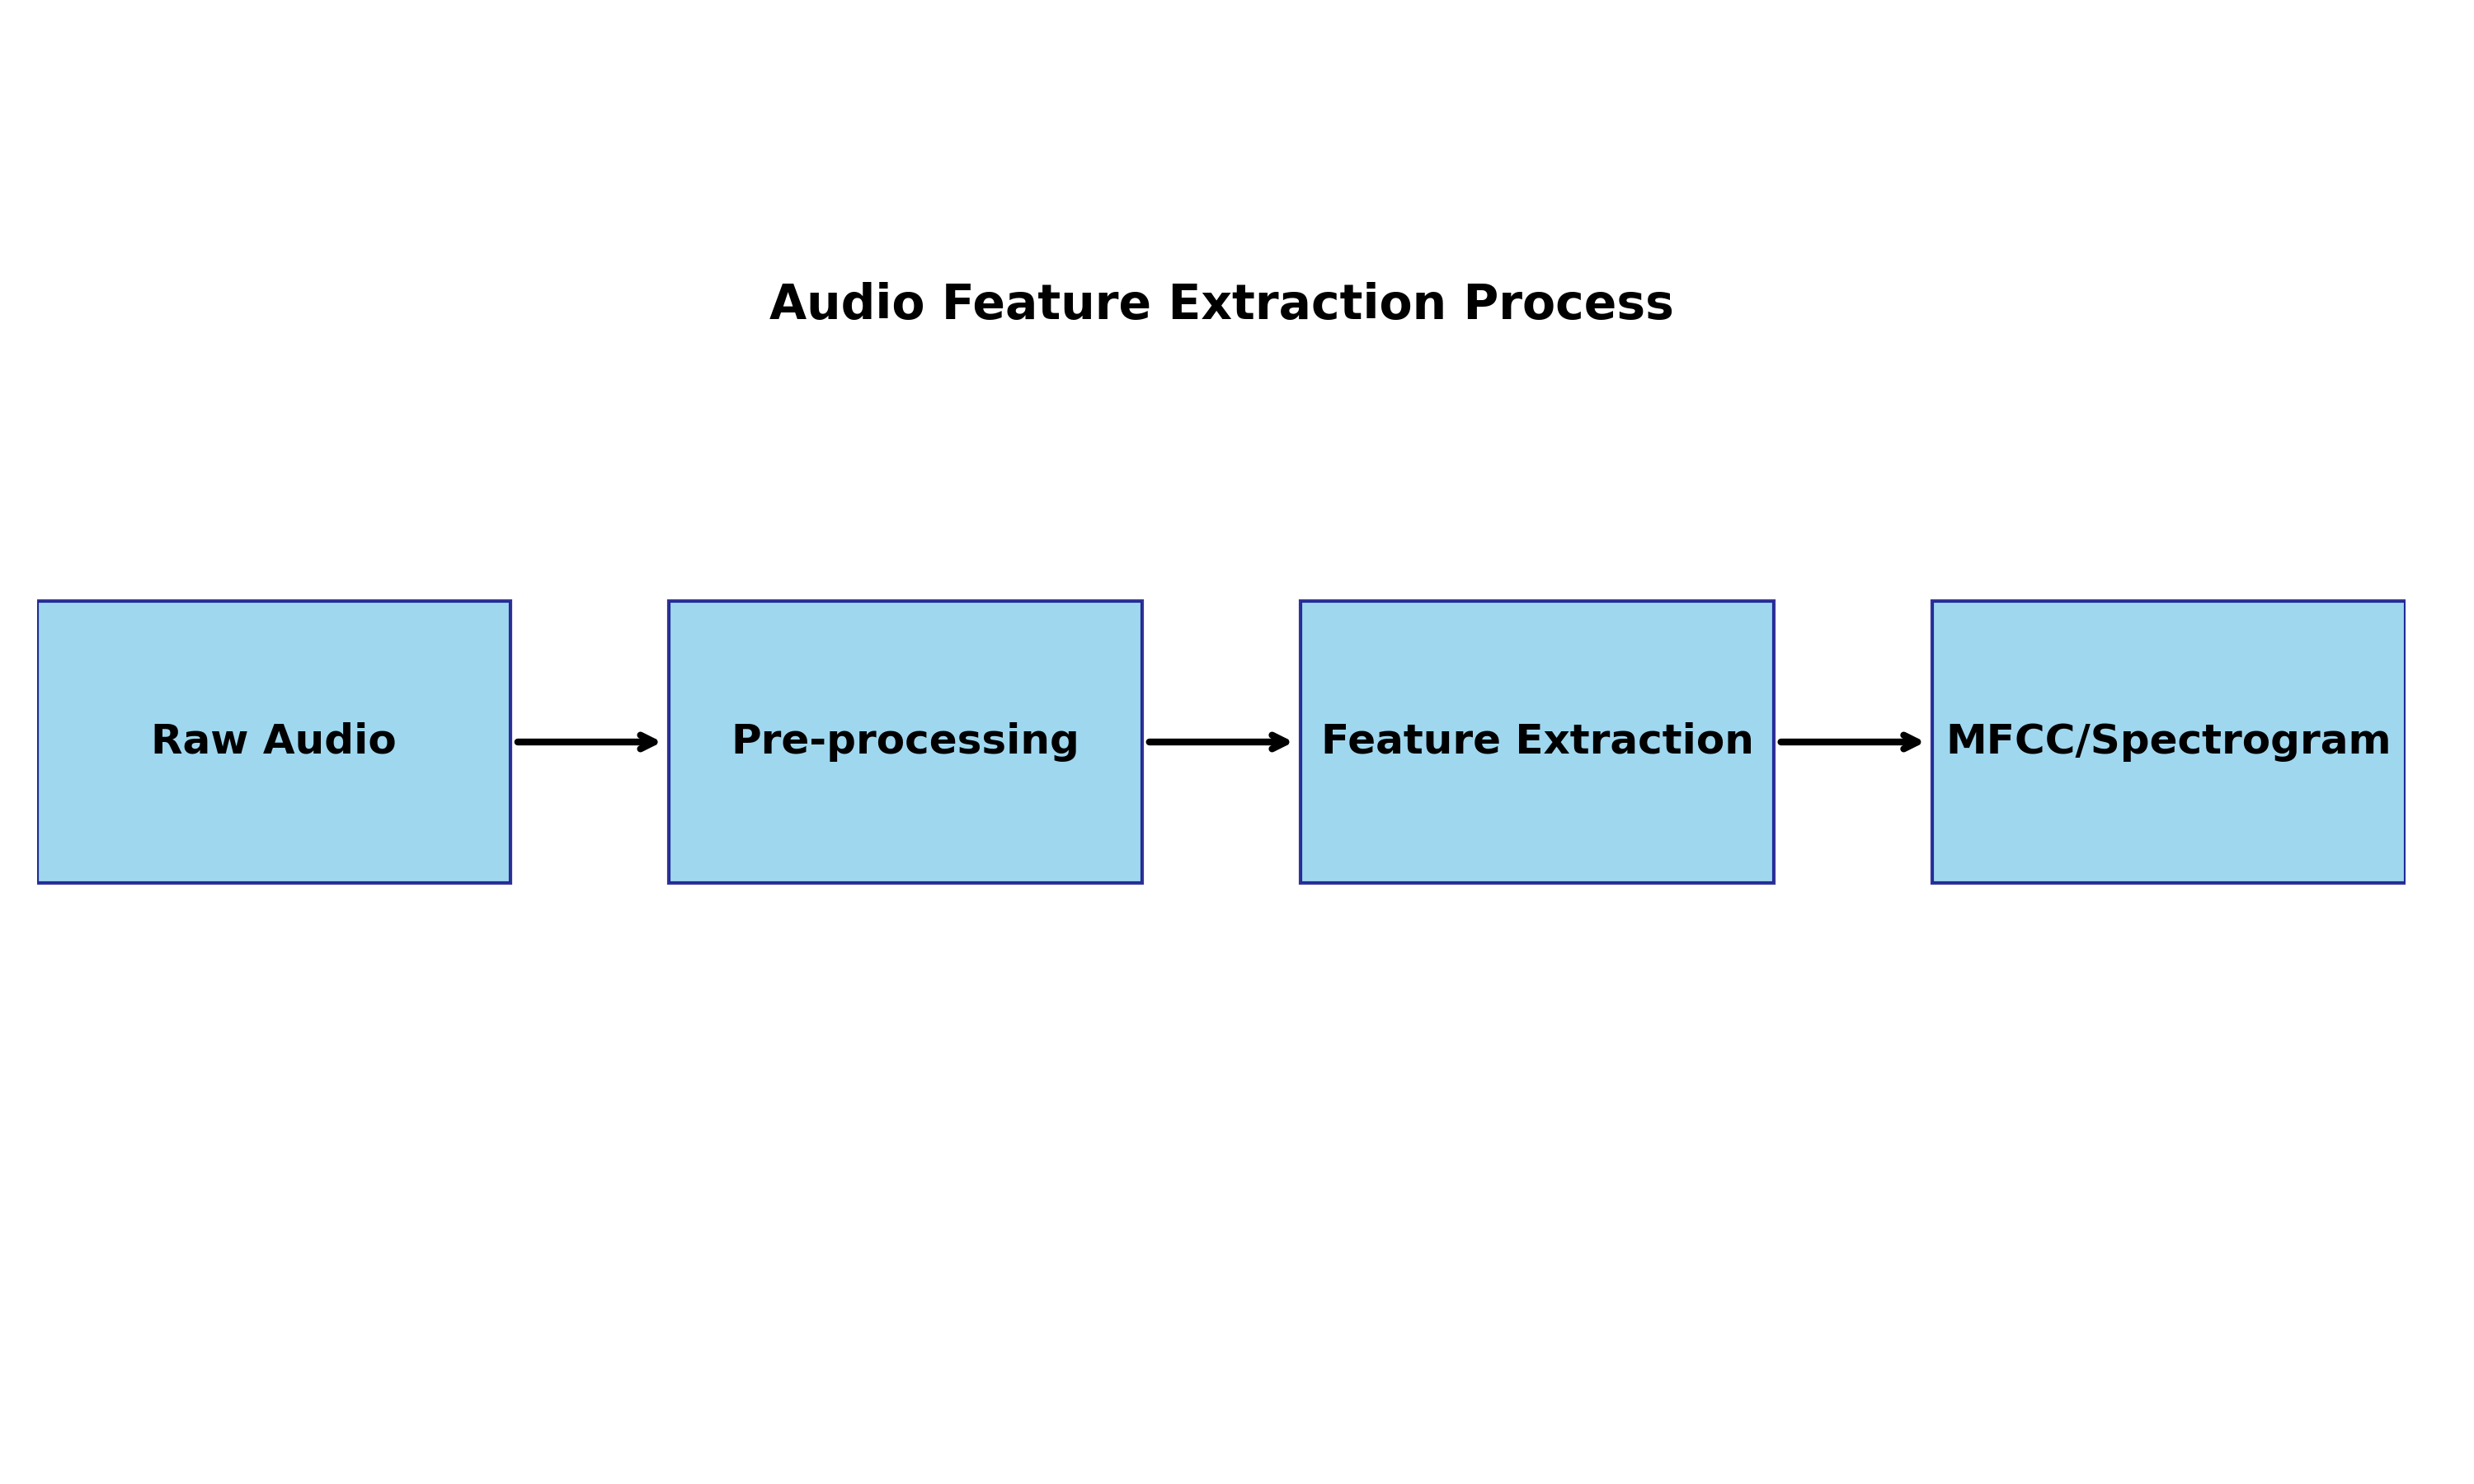
\includegraphics[width=0.9\textwidth]{figures/audio_feature_extraction.png}
\end{center}

\begin{itemize}
    \item \textbf{MFCCs}: Mel-Frequency Cepstral Coefficients (vocal tract characteristics)
    \item \textbf{Spectrograms}: Visual representation of spectrum of frequencies
    \item \textbf{Prosodic Features}: Pitch, energy, speaking rate, rhythm
    \item \textbf{Wav2vec Embeddings}: Self-supervised audio representations
\end{itemize}
\end{frame}

\begin{frame}
\frametitle{MFCC Extraction Process}
\begin{columns}
\column{0.6\textwidth}
\begin{enumerate}
    \item \textbf{Pre-emphasis}: Apply high-pass filter to amplify high frequencies
    \item \textbf{Framing}: Divide signal into short frames (20-40ms)
    \item \textbf{Windowing}: Apply Hamming window to each frame
    \item \textbf{FFT}: Calculate power spectrum using Fast Fourier Transform
    \item \textbf{Mel Filtering}: Apply mel-scale filterbank (mimics human hearing)
    \item \textbf{Log Compression}: Take logarithm of filter outputs
    \item \textbf{DCT}: Discrete Cosine Transform to decorrelate features
    \item \textbf{Feature Selection}: Keep 13-20 coefficients
\end{enumerate}

\column{0.4\textwidth}
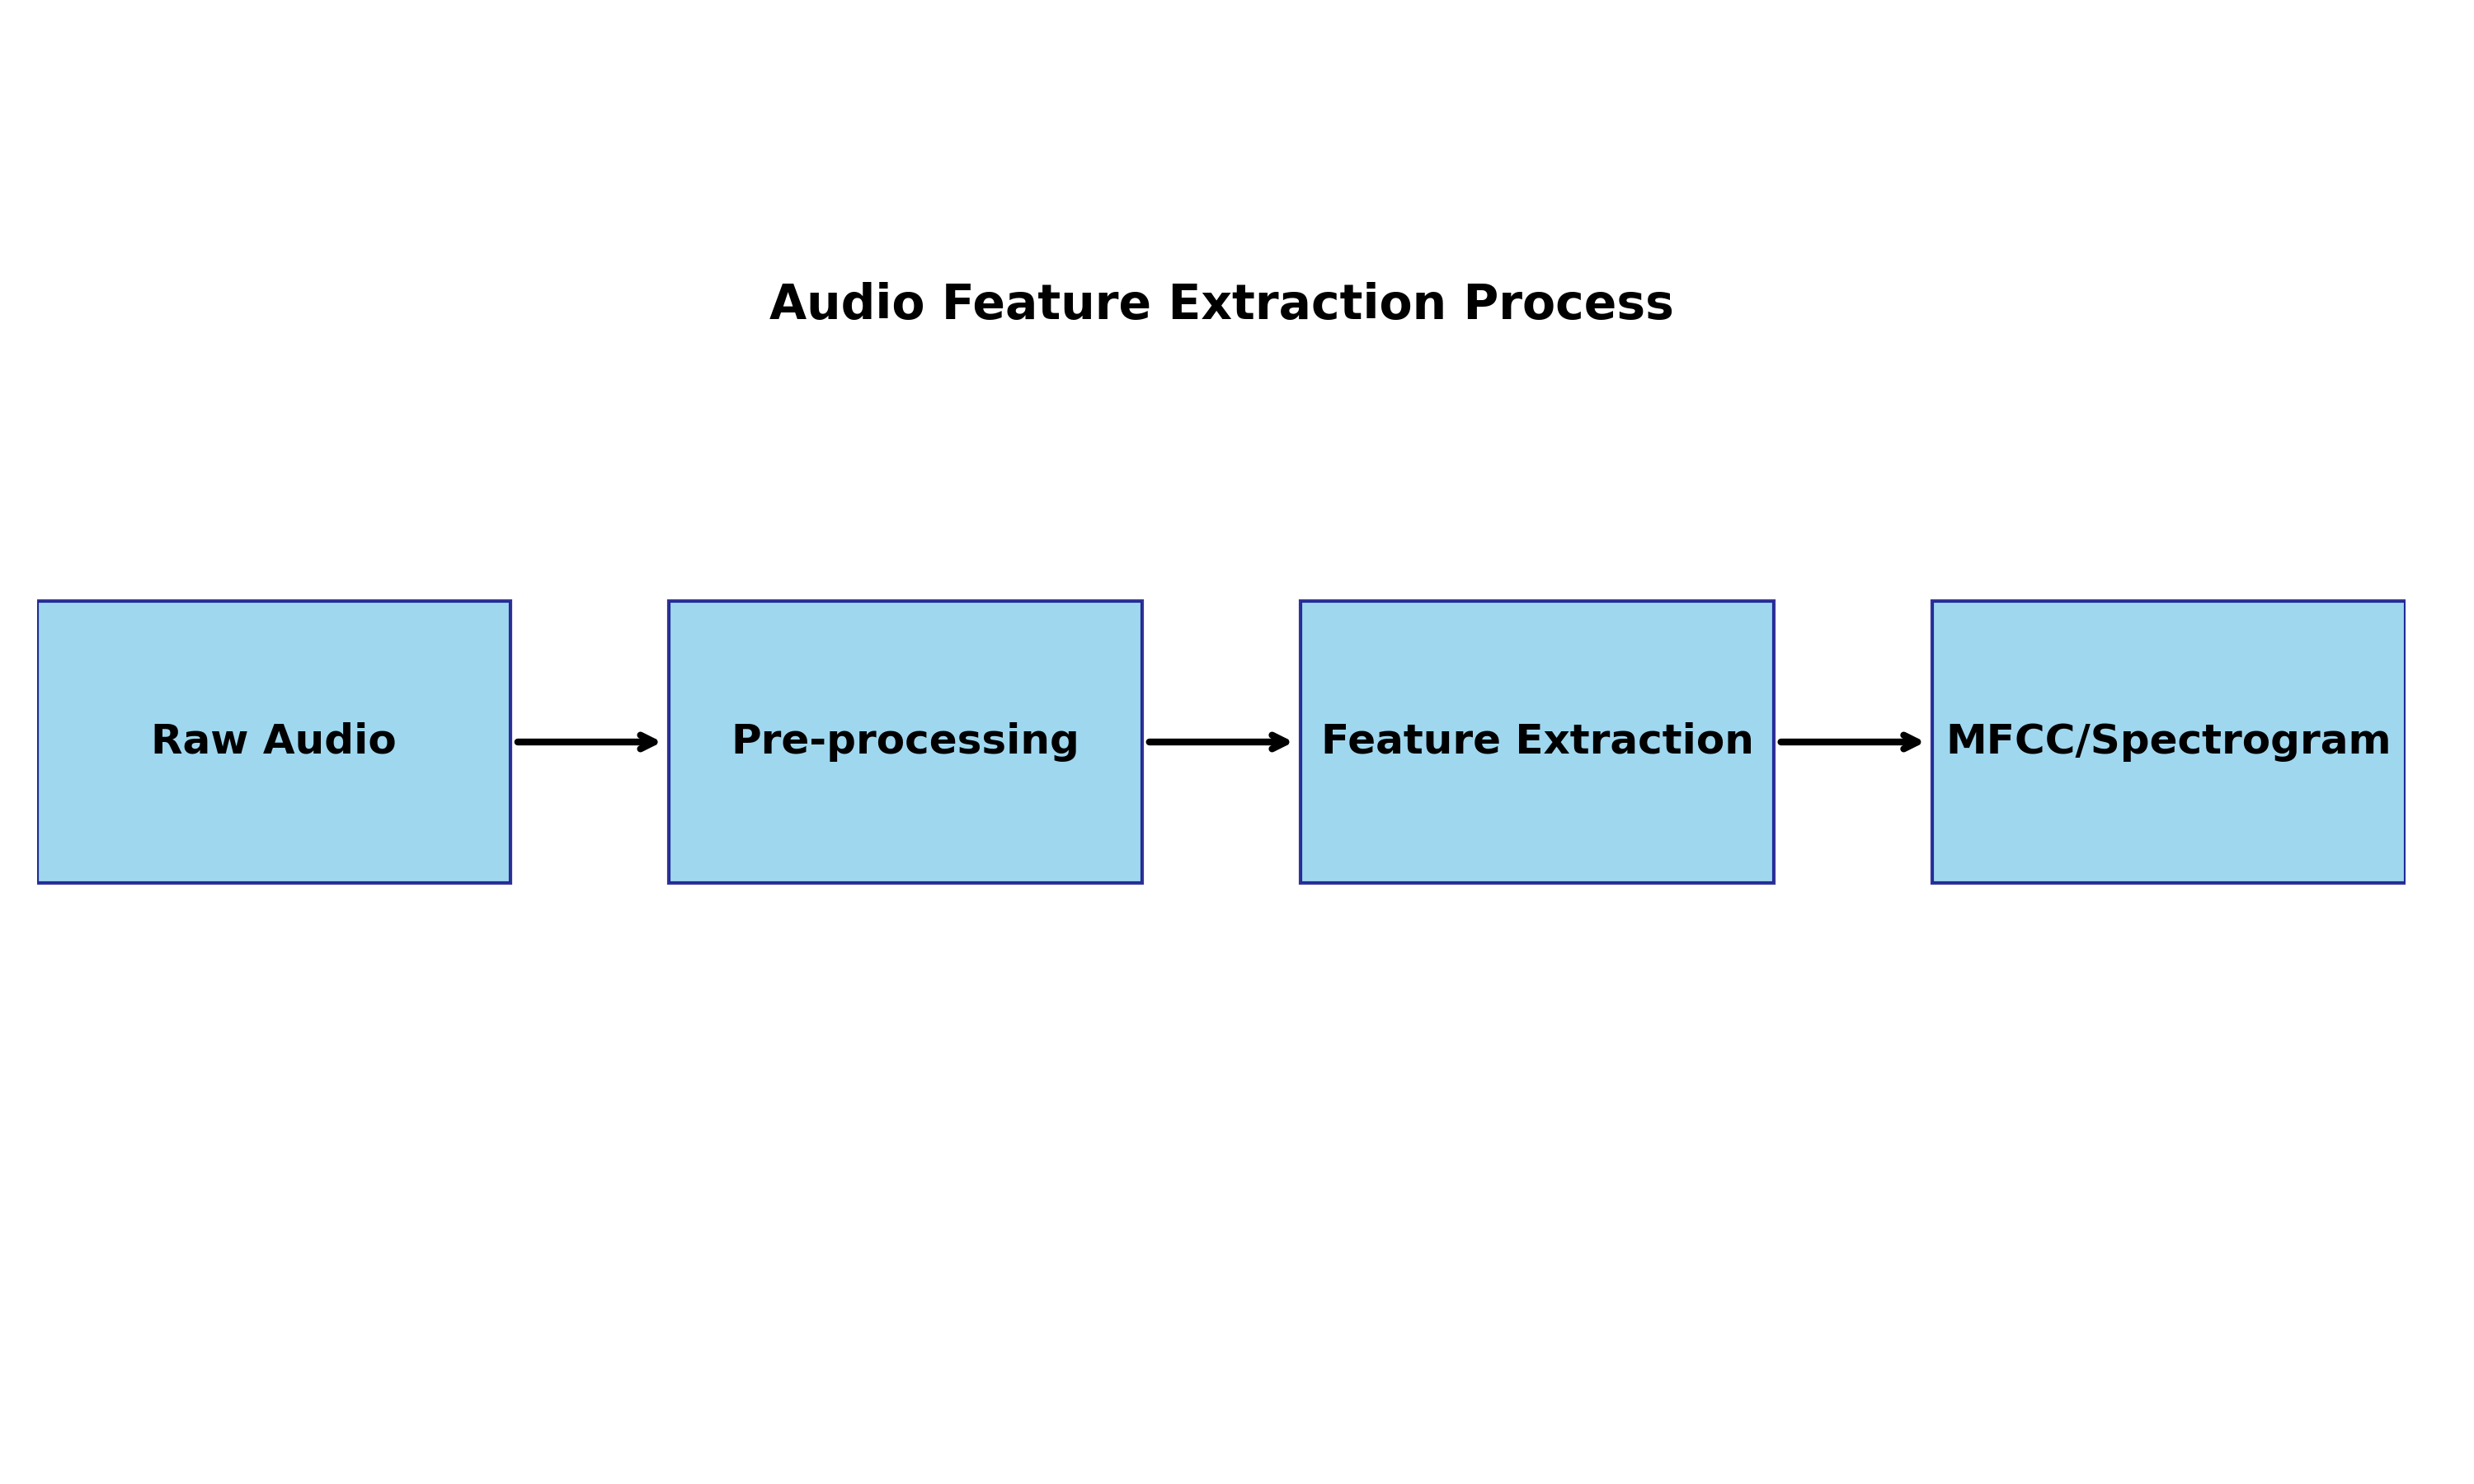
\includegraphics[width=\textwidth]{figures/audio_feature_extraction.png}
\end{columns}

\begin{itemize}
    \item \textbf{Implementation}: Librosa library with 40ms windows, 10ms step
    \item \textbf{Parameters}: 40 mel-filters, 13 MFCCs + delta + delta-delta features
\end{itemize}
\end{frame}

\begin{frame}
\frametitle{Wav2Vec Embeddings}
\begin{itemize}
    \item \textbf{Self-supervised Learning for Audio}:
    \begin{itemize}
        \item Pre-trained on 960 hours of LibriSpeech
        \item Learns representations from raw audio
        \item No need for labeled data during pre-training
    \end{itemize}
    \item \textbf{Architecture}:
    \begin{itemize}
        \item Encoder: Extracts features from raw audio
        \item Context Network: Captures contextual information
        \item Contrastive task: Predicts future audio segments
    \end{itemize}
    \item \textbf{Advantages}:
    \begin{itemize}
        \item Captures subtle acoustic patterns
        \item More robust to background noise
        \item Transfer learning benefits
        \item Strong performance on emotional content
    \end{itemize}
\end{itemize}
\end{frame}

\begin{frame}
\frametitle{Fusion Strategies}
\begin{center}
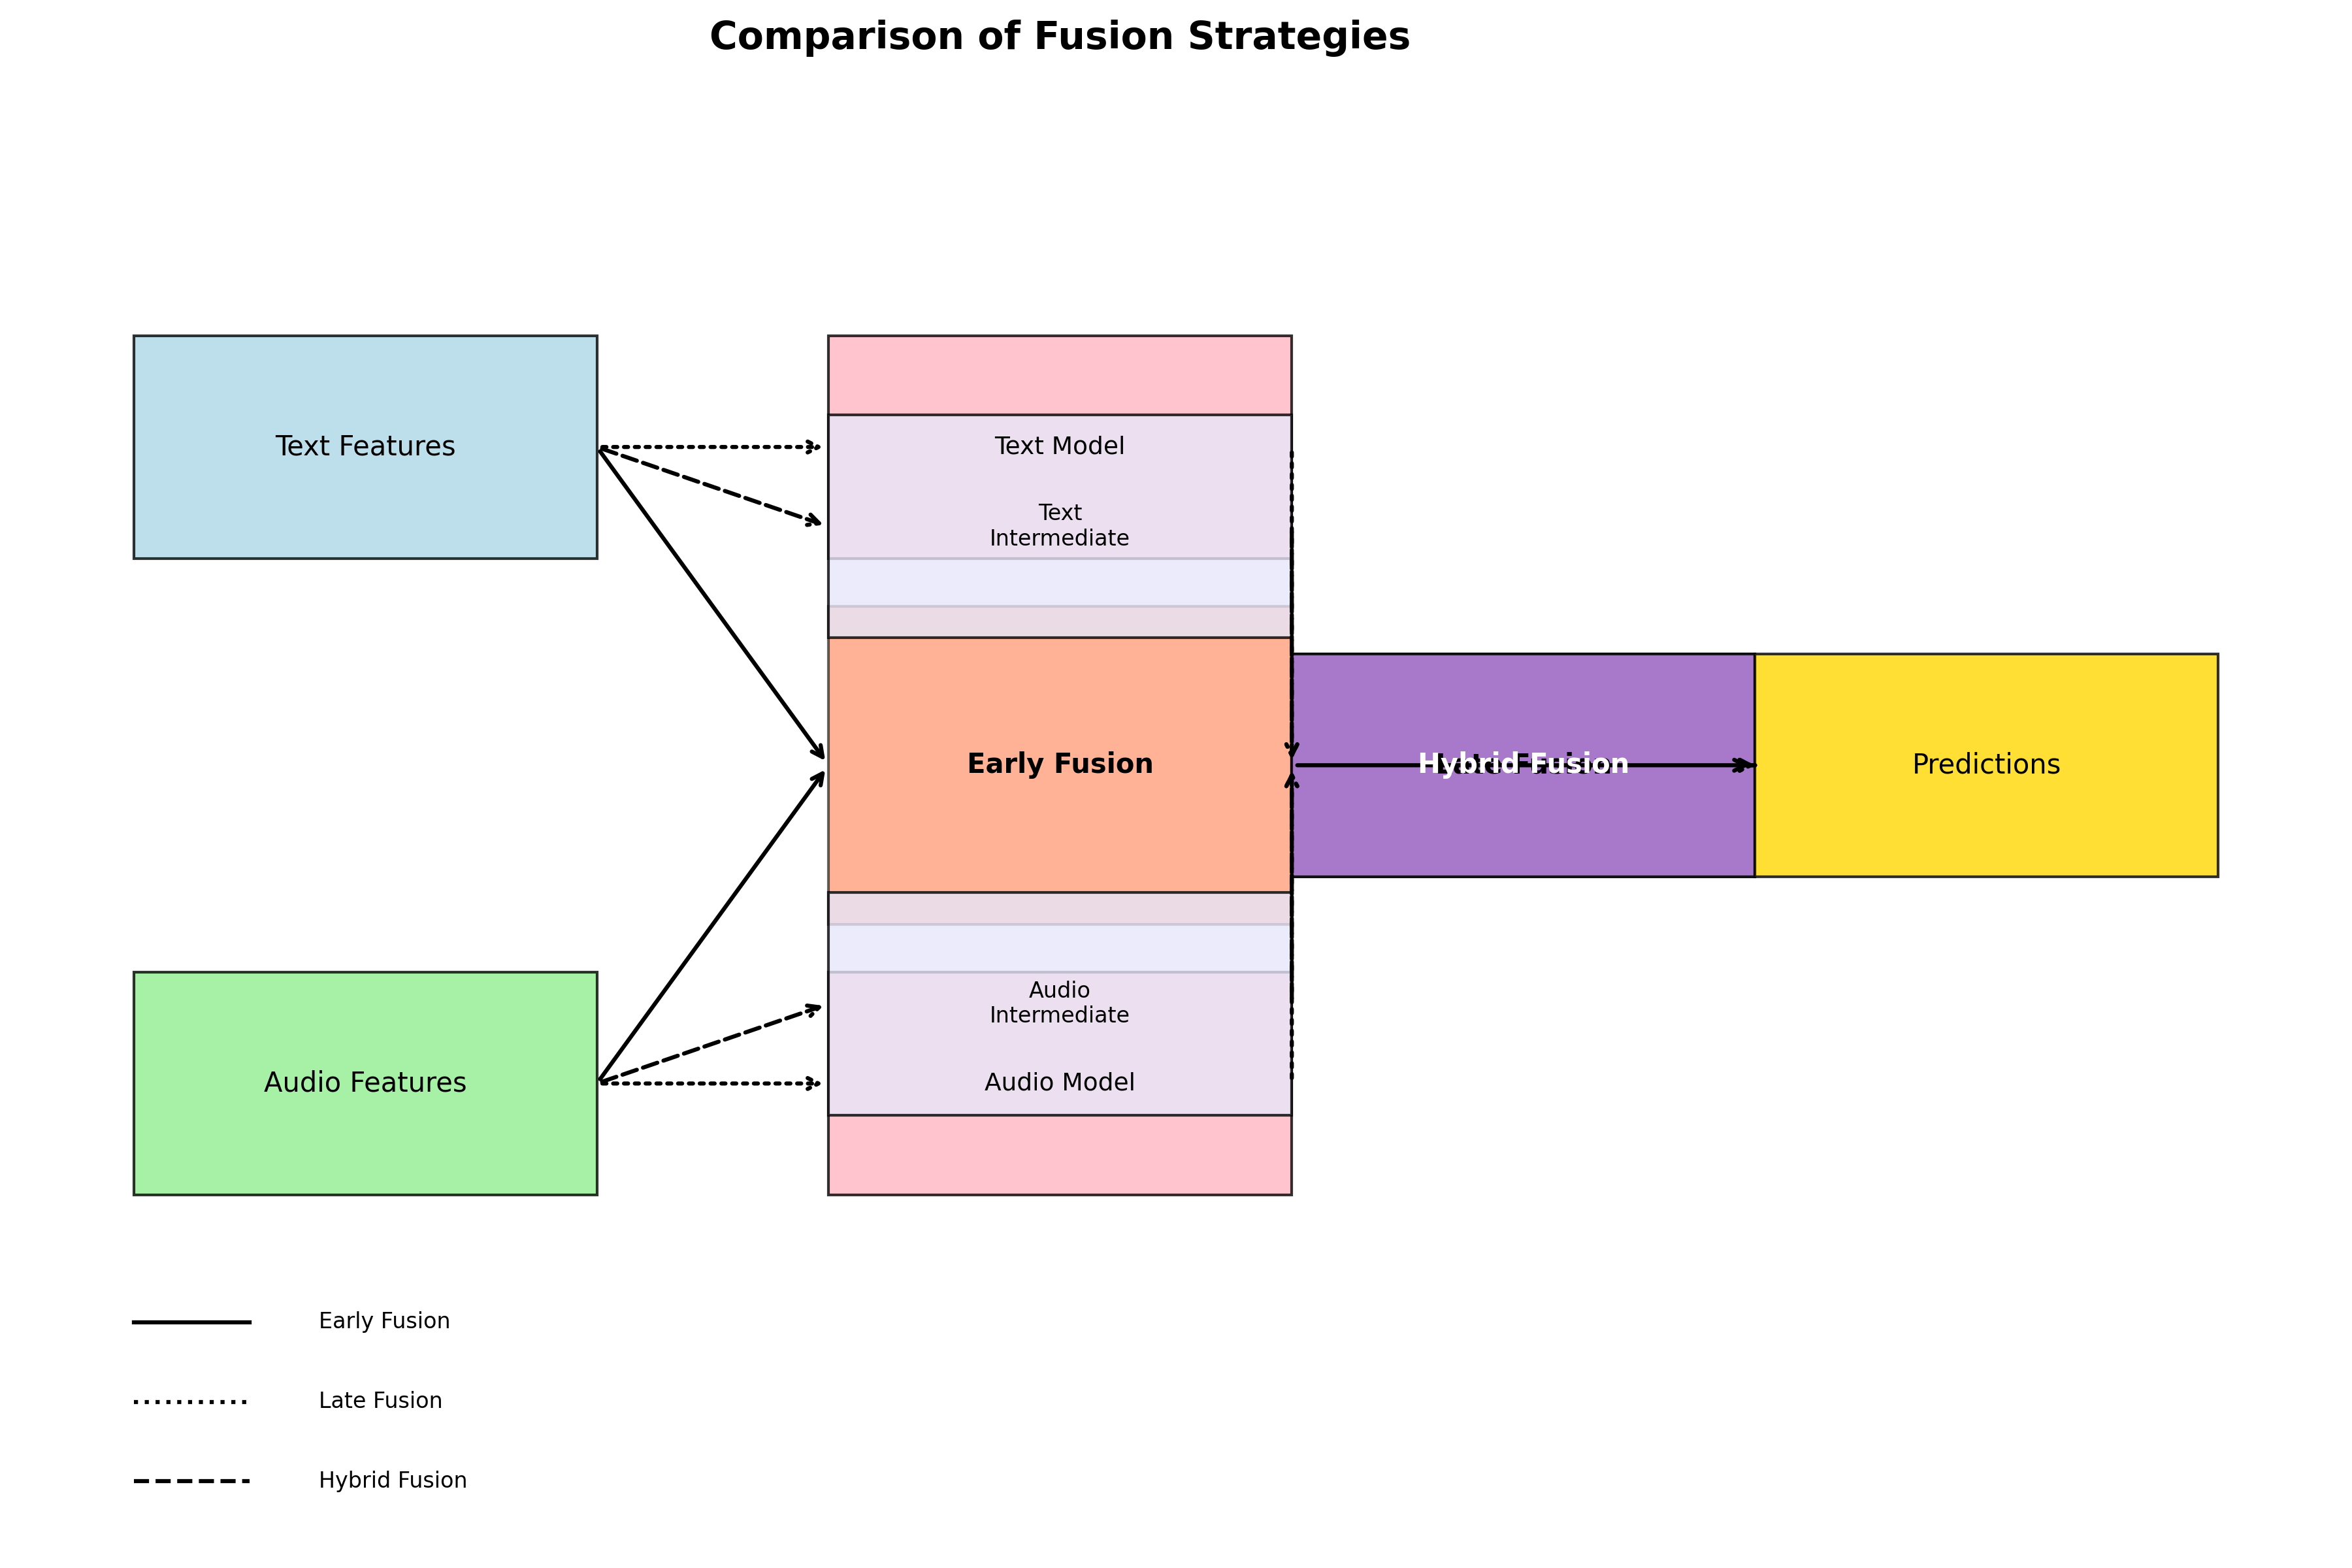
\includegraphics[width=0.9\textwidth]{figures/fusion_strategies.png}
\end{center}

\begin{itemize}
    \item \textbf{Early Fusion}: Combine raw features before processing
    \item \textbf{Late Fusion}: Process modalities independently, combine predictions
    \item \textbf{Hybrid Fusion}: Combine at intermediate processing stages
    \item \textbf{Attention-Based Fusion}: Dynamic weighting based on importance
\end{itemize}
\end{frame}

\begin{frame}
\frametitle{Early Fusion Details}
\begin{columns}
\column{0.5\textwidth}
\begin{itemize}
    \item \textbf{Process}:
    \begin{itemize}
        \item Extract features from each modality
        \item Concatenate feature vectors
        \item Process combined features through joint model
    \end{itemize}
    \item \textbf{Advantages}:
    \begin{itemize}
        \item Captures low-level interactions
        \item Single model to train
        \item Potentially better feature interactions
    \end{itemize}
\end{itemize}

\column{0.5\textwidth}
\begin{itemize}
    \item \textbf{Challenges}:
    \begin{itemize}
        \item Requires compatible feature dimensions
        \item Dominated by higher-dimensional modality
        \item Synchronization issues
        \item Less modality-specific optimization
    \end{itemize}
    \item \textbf{Implementation}:
    \begin{itemize}
        \item Feature normalization
        \item Dimension matching via projection
        \item Joint training
    \end{itemize}
\end{itemize}
\end{columns}
\end{frame}

\begin{frame}
\frametitle{Late Fusion Details}
\begin{columns}
\column{0.6\textwidth}
\begin{itemize}
    \item \textbf{Process}:
    \begin{itemize}
        \item Train separate models for each modality
        \item Extract predictions from each model
        \item Combine predictions using:
        \begin{itemize}
            \item Weighted averaging
            \item Voting mechanisms
            \item Meta-learner (stacking)
        \end{itemize}
    \end{itemize}
    \item \textbf{Advantages}:
    \begin{itemize}
        \item Modality-specific optimization
        \item Easier to handle missing modalities
        \item Simpler implementation
    \end{itemize}
\end{itemize}

\column{0.4\textwidth}
\begin{itemize}
    \item \textbf{Challenges}:
    \begin{itemize}
        \item Misses cross-modal interactions
        \item Potential redundancy in learning
        \item Higher computational cost
    \end{itemize}
    \item \textbf{Implementation}:
    \begin{itemize}
        \item Grid search for optimal weights
        \item Cross-validation for meta-learner
        \item Bayesian optimization
    \end{itemize}
\end{itemize}
\end{columns}
\end{frame}

\begin{frame}
\frametitle{Hybrid and Attention-Based Fusion}
\begin{columns}
\column{0.5\textwidth}
\textbf{Hybrid Fusion}:
\begin{itemize}
    \item Combines early and late fusion approaches
    \item Extract intermediate representations
    \item Fuse at multiple levels of abstraction
    \item Benefits:
    \begin{itemize}
        \item Captures both low and high-level interactions
        \item Balances modality-specific and joint learning
        \item More flexible architecture
    \end{itemize}
\end{itemize}

\column{0.5\textwidth}
\textbf{Attention-Based Fusion}:
\begin{itemize}
    \item Uses attention mechanisms to weight modalities
    \item Learns importance of each modality dynamically
    \item Can be applied at different levels
    \item Benefits:
    \begin{itemize}
        \item Adaptive weighting based on input
        \item Better handling of noisy modalities
        \item Improved interpretability
    \end{itemize}
\end{itemize}
\end{columns}

\begin{itemize}
    \item \textbf{Our Implementation}: Cross-modal attention between text and audio features
\end{itemize}
\end{frame}

\begin{frame}
\frametitle{Computational Resources}
\begin{columns}
\column{0.5\textwidth}
\begin{itemize}
    \item \textbf{Computing Infrastructure}:
    \begin{itemize}
        \item \alert{10 NVIDIA H100 GPUs} via Modal.com
        \item 80GB VRAM per GPU
        \item NVLink interconnect
    \end{itemize}
    \item \textbf{Experiment Scale}:
    \begin{itemize}
        \item \alert{392 total experiments}
        \item 1,500+ GPU hours
        \item 6 text models × 4 audio features × 4 fusion strategies
    \end{itemize}
\end{itemize}

\column{0.5\textwidth}
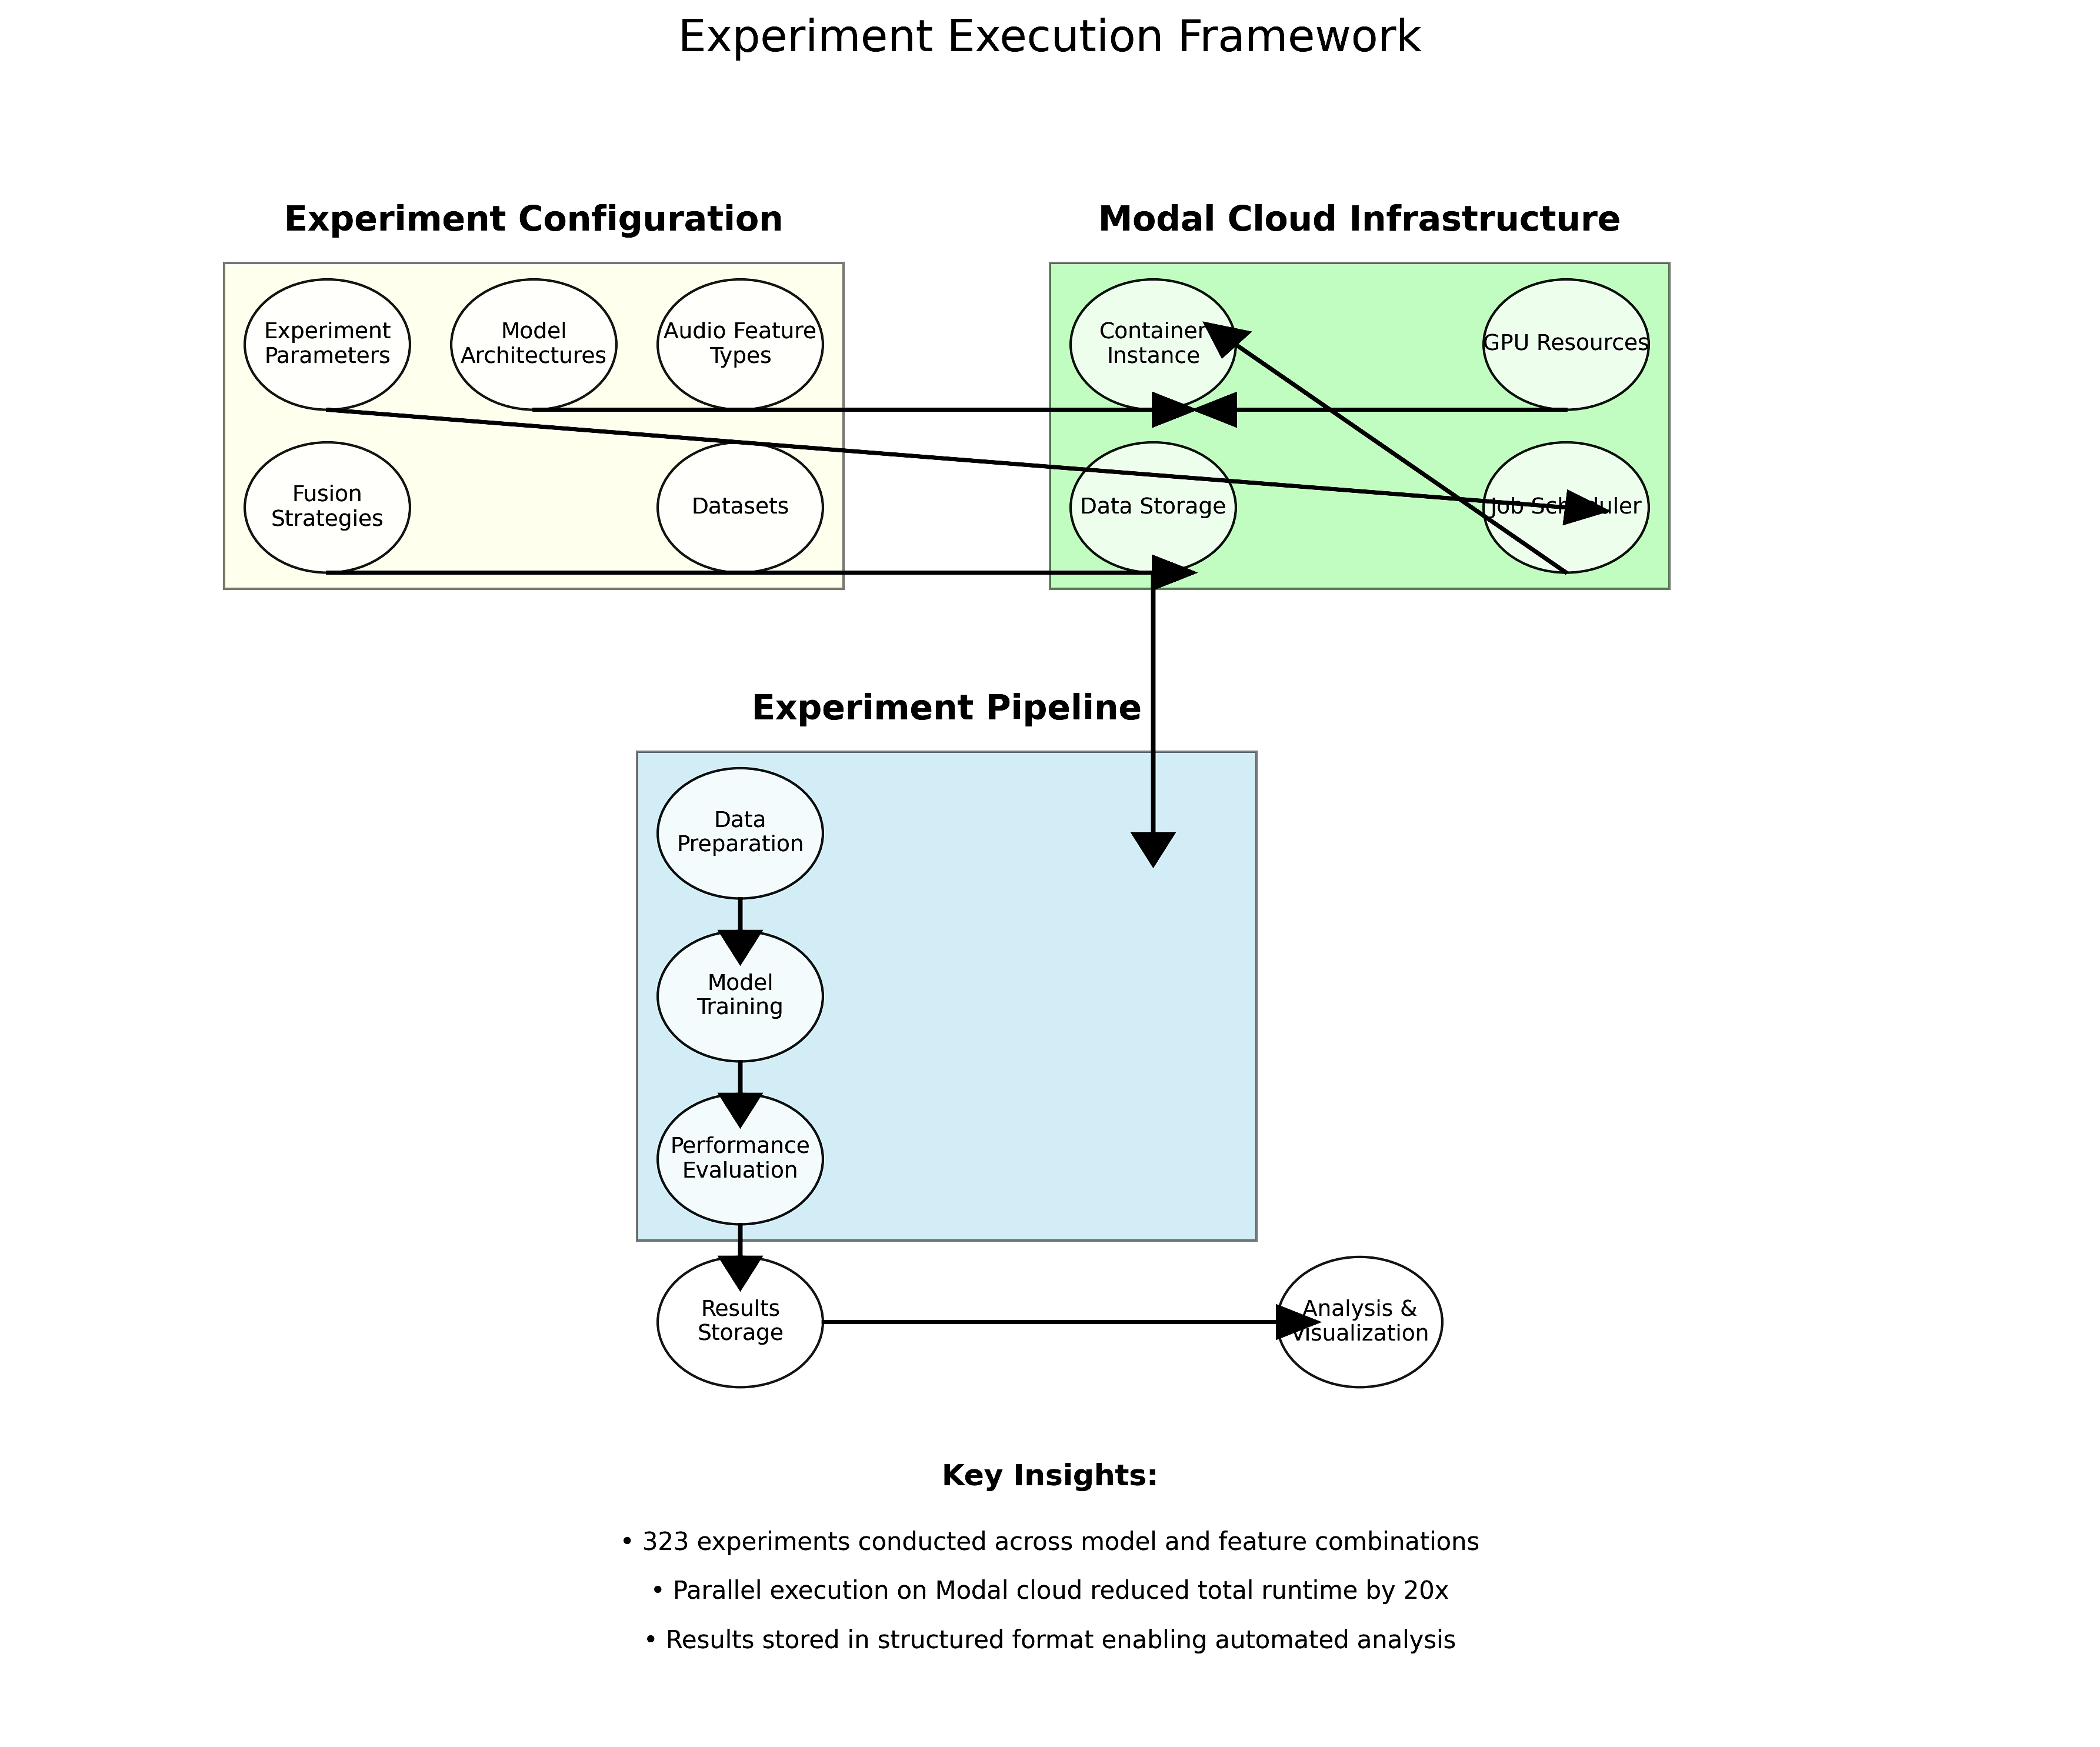
\includegraphics[width=\textwidth]{figures/experiment_framework.png}
\end{columns}
\end{frame}

\begin{frame}
\frametitle{Experiment Matrix}
\begin{itemize}
    \item \textbf{6 Text Models} × \textbf{4 Audio Feature Types} × \textbf{4 Fusion Strategies} × \textbf{2 Approaches}:
    \begin{itemize}
        \item \textbf{Text Models}: BERT, RoBERTa, XLNet, ALBERT, ELECTRA, DeBERTa
        \item \textbf{Audio Features}: MFCCs, Spectrograms, Prosodic Features, Wav2vec
        \item \textbf{Fusion Strategies}: Early, Late, Hybrid, Attention-based
        \item \textbf{Approaches}: Direct Classification, Two-Stage
    \end{itemize}
    \item Plus single-modality experiments and ablation studies
    \item Model training with 5-fold cross-validation
    \item Each experiment repeated 3 times with different random seeds
\end{itemize}
\end{frame}

\begin{frame}
\frametitle{Dataset: IEMOCAP}
\begin{columns}
\column{0.6\textwidth}
\begin{itemize}
    \item \textbf{Interactive Emotional Dyadic Motion Capture database}
    \item 12 hours of audio-visual data
    \item 10 actors (5 male, 5 female) in dyadic sessions
    \item \textbf{Annotation}:
    \begin{itemize}
        \item Categorical: anger, happiness, sadness, neutral, surprise, fear, disgust
        \item Dimensional: valence, arousal, dominance (1-5 scale)
    \end{itemize}
    \item \textbf{Content}:
    \begin{itemize}
        \item Scripted scenarios
        \item Improvised scenarios based on situations
        \item 10,039 utterances total
    \end{itemize}
\end{itemize}

\column{0.4\textwidth}
\begin{itemize}
    \item \textbf{Data Distribution}:
    \begin{itemize}
        \item Anger: 1,103 (19.5\%)
        \item Happiness: 1,636 (29.0\%)
        \item Sadness: 1,084 (19.2\%)
        \item Neutral: 1,708 (30.3\%)
        \item Others: 110 (2.0\%)
    \end{itemize}
    \item \textbf{Data Split}:
    \begin{itemize}
        \item Training: 70\%
        \item Validation: 15\%
        \item Testing: 15\%
        \item Speaker-independent split
    \end{itemize}
\end{itemize}
\end{columns}
\end{frame}

\begin{frame}
\frametitle{Evaluation Metrics}
\begin{columns}
\column{0.5\textwidth}
\textbf{For Categorical Classification}:
\begin{itemize}
    \item Accuracy
    \item Precision, Recall, F1-score
    \item Macro and Micro averaging
    \item Confusion matrices
\end{itemize}

\textbf{For Dimensional Prediction}:
\begin{itemize}
    \item Mean Absolute Error (MAE)
    \item Root Mean Squared Error (RMSE)
    \item Coefficient of Determination (R²)
    \item Concordance Correlation Coefficient (CCC)
\end{itemize}

\column{0.5\textwidth}
\textbf{For Comparative Analysis}:
\begin{itemize}
    \item Statistical significance tests
    \item Ablation studies
    \item Performance vs. complexity
    \item Error analysis
\end{itemize}

\textbf{For Fusion Assessment}:
\begin{itemize}
    \item Relative performance gain
    \item Modality contribution analysis
    \item Computational efficiency
    \item Robustness to noise/missing data
\end{